\documentclass{article}

\usepackage{epsfig}
\usepackage[mathscr]{eucal}
\usepackage{amsfonts}
\usepackage{amscd}
\usepackage{amsmath}
\usepackage{array}
\usepackage{amssymb}
%\usepackage[backend=bibtex8, sorting=none]{biblatex}
\usepackage{colordvi}
\usepackage{enumerate}
\usepackage{graphicx}
\usepackage{here}
\usepackage{booktabs}
\usepackage[footnotesize]{caption}
\usepackage{fancyhdr}
\usepackage{pdfpages}
\usepackage{slashed}
\usepackage{tabularx}
\usepackage{longtable}
\usepackage{array}
\usepackage{caption}
\usepackage{subcaption}

%\usepackage{relsize}
\usepackage{color}
\usepackage{rotating}

\usepackage{slashed}

\usepackage{epsfig,amsmath,graphicx,amssymb,listings,slashed}
\usepackage[colorlinks,citecolor=blue,urlcolor=blue,linkcolor=blue]{hyperref}
\usepackage[outercaption]{sidecap}

\usepackage{booktabs}

%\smartqed
%\usepackage[T1]{fontenc}
\usepackage[utf8]{inputenc}

\usepackage{epsfig,amsmath,graphicx,amssymb,listings,slashed}
\usepackage[colorlinks,citecolor=blue,urlcolor=blue,linkcolor=blue]{hyperref}

\setlength{\evensidemargin}{0cm}
\setlength{\oddsidemargin}{0cm}
\setlength{\topmargin}{0.00cm}
\setlength{\textwidth}{16.0cm}
\setlength{\textheight}{24.00cm}
\setlength{\headheight}{0cm}
\setlength{\headsep}{0cm}
\setlength{\voffset}{0cm}
\setlength{\paperheight}{29cm}

\definecolor{ourbrown}{RGB}{155,100,15}
\definecolor{ourcyan}{RGB}{20,165,165}
\definecolor{ourpurple}{RGB}{145,0,140}
\definecolor{darkorange}{RGB}{225,100,0}
\definecolor{darkgreen}{RGB}{0,170,0}
\definecolor{darkgray}{RGB}{80,80,80}

\setlength{\marginparwidth}{20mm}

%\bibliography{literature.bib}





\begin{document}

\title{ Machine Learning - SS 2021 \\ Exercise 1: Classification }


	\author{Federico Ambrogi, \textcolor{blue} {e1449911@student.tuwien.ac.at } \\
	Adam Höfler, \textcolor{blue} {e11847620@student.tuwien.ac.at } \\
	Matteo Panzeri \textcolor{blue}{12039996@student.tuwien.ac.at } \\
    TU Wien }


%\ead{federico.ambrogi@univie.ac.at}




\maketitle
\setcounter{tocdepth}{2}
\tableofcontents

\section{Introduction}
In this document we describe the results of the implementation of three algorithms to solve classification problems on four different dataset. we will first briefly describe the datasets we will classify; then, the framework and the algorithms chosen for the classification task are introduced. A brief description of the data pre-processing is then given. Finally, the results of the classifications as well as a few comparisons between different settings are discussed. 




\subsection{Data Sets Description}
Here we briefly introduce our four datasets.

\paragraph{Drug consumption data set} This is the data set taken from exercise 0, so here we only provide basic details. The primary task of our implementation is to classify the likeliness of the frequency of usage of a certain type of drug (from never used to current usage), given personal aspects such as gender, ethnicity, education background etc. and psychological traits.
In detail:
\begin{itemize}
	\item  \textbf{attributes}: 'age', 'gender', 'education', 'ethnicity', 'Nscore', 'Escore', 'Oscore', 'Ascore', 'Cscore', 'Impulsive', 'SS' \\
	\item  \textbf{targets}: 'alcohol', 'amphetamines', 'amylNitrite', 'benzodiazepine', 'caffeine', 'cannabis', 'chocolate', 'cocaine', 'crack', 'ecstasy', 'heroin', 'ketamine', 'legal', 'LSD',
	'methadone', 'mushrooms', 'nicotine', 'volatileSubstance'
	divided in \textbf{7 classes}: "Never", ">10 Years Ago", "Last Decade", "Last Year", "Last Month", "Last Week", "Last Day"
\end{itemize}


\paragraph{Asteroids data set}
The asteroids data set is designed to perform a binary classification task. It consists of a total of astrophysical data, such as the distance from the Earth, the size of the major axis of the orbits, their mass etc. as well metadata regarding their name. The target feature for classification is a string variable that maps to boolean values "True" in the case the asteroid represents a concrete hazard for the Earth i.e. with high risk of impact, and "False" otherwise.

In detail:
\begin{itemize}
	\item  \textbf{attributes}:'Absolute Magnitude', 'Est Dia in KM(min)', 'Est Dia in KM(max)', 'Relative Velocity km per sec', 'Miss Dist.(kilometers)', 'Minimum Orbit Intersection', 'Jupiter Tisserand Invariant', 'Eccentricity', 'Semi Major Axis', 'Inclination', 'Asc Node Longitude', 'Orbital Period', 'Perihelion   Distance', 'Perihelion Arg', 'Aphelion Dist', 'Perihelion Time', 'Mean Anomaly', 'Mean Motion' \\


	\item  \textbf{target}: 'Hazardous' divided in \textbf{classes}: "True" and "False" \\
\end{itemize}


\paragraph{Breast Cancer (Kaggle Data Set)}
ccc

\begin{itemize}
	\item  \textbf{attributes}: 'radiusMean', 'textureMean', 'perimeterMean', 'areaMean',
	'smoothnessMean', 'compactnessMean', 'concavityMean',
	'concavePointsMean', 'symmetryMean', 'fractalDimensionMean',
	'radiusStdErr', ' textureStdErr' ,'perimeterStdErr' ,'areaStdErr',
	'smoothnessStdErr', 'compactnessStdErr', 'concavityStdErr',
	'concavePointsStdErr' ,'symmetryStdErr' ,'fractalDimensionStdErr',
	'radiusWorst', 'textureWorst' ,'perimeterWorst' ,'areaWorst',
	'smoothnessWorst' ,'compactnessWorst' ,'concavityWorst',
	'concavePointsWorst', 'symmetryWorst', 'fractalDimensionWorst' \\

	\item  \textbf{target}: 'class' divided in \textbf{classes}: "True" and "False" \\
\end{itemize}

\paragraph{Advertising Bidding (Kaggle Data Set)}

In detail:
\begin{itemize}
	\item  \textbf{attributes}: 'Region', 'City', 'AdExchange', 'Adslotwidth', 'Adslotheight', 'Adslotfloorprice',
	'CreativeID', 'Biddingprice', 'AdvertiserID', 'interest\_news', 'eduation', 'automobile','interest\_realestate', 'IT', 'electronicgame','interest\_fashion', 'entertainment', 'luxury','homeandlifestyle', 'interest\_health', 'food','interest\_divine', 'interest\_motherhood\_parenting', 'sports','interest\_travel\_outdoors', 'interest\_social', 'Inmarket\_3cproduct','Inmarket\_appliances', 'Inmarket\_clothing\_shoes\_bags' ,

	'Inmarket\_Beauty\_PersonalCare', 'Inmarket\_infant\_momproducts',
	'Inmarket\_sportsitem', 'Inmarket\_outdoor', 'Inmarket\_healthcareproducts',
	'Inmarket\_luxury', 'Inmarket\_realestate',

	'Inmarket\_automobile',
	'Inmarket\_finance', 'Inmarket\_travel', 'Inmarket\_education',
	'Inmarket\_service', 'art\_photography\_design',
	'onlineliterature', 'Inmarket\_electronicgame', '3c',
	'Inmarket\_book', 'Inmarket\_medicine', 'Inmarket\_fooddrink',
	'culture', 'sex',
	'Demographic\_gender\_male',

	'Demographic\_gender\_famale', 'Inmarket\_homeimprovement', 'Payingprice',
	'imp', 'click', 'Browser', 'Adslotvisibility', 'Adslotformat' \\

	\item  \textbf{target}: 'conv' divided in \textbf{classes}: "True" and "False"
\end{itemize}

In detail:
\begin{itemize}
	\item  \textbf{attributes}:'Absolute Magnitude', 'Est Dia in KM(min)', 'Est Dia in KM(max)', 'Relative Velocity km per sec', 'Miss Dist.(kilometers)', 'Minimum Orbit Intersection', 'Jupiter Tisserand Invariant', 'Eccentricity', 'Semi Major Axis', 'Inclination', 'Asc Node Longitude', 'Orbital Period', 'Perihelion   Distance', 'Perihelion Arg', 'Aphelion Dist', 'Perihelion Time', 'Mean Anomaly', 'Mean Motion' \\

	\item  \textbf{target}: 'Hazardous' divided in \textbf{classes}: "True" and "False"
\end{itemize}

\subsection{Framework and Implementation}
We implemented our analysis using the \textbf{python3.8} language, with its library for machine learning application \textit{scikit-learn} as well as \textit{numpy} and \textit{pandas} for data statistical analysis and data manipulation. In the attached package, two distinct files can be found: the first, called \textit{data\_preparation.py}, cleans and standardizes the input data set, so that they are ready for data processing. The main script for the data analysis is called \textit{classifier.py}. This code will run the different classifiers on the data sets, and will produce the comparison data and plots that will be found in this report.


\subsection{Workflow Overview}
Without giving particular details on the implementations of the various classifier, which can be read inside the scripts, we summarize here how the workflow is constructed, as well as how the classification tasks have been implemented.
First, the cleaned data (i.e. processed by \textit{data\_preparation.py} ) are imported as \textit{pandas} data frame. For each data set, a dictionary provided the list of names of features that will be used to predict the target feature. Then, we analyse the class balancing of the predicting features; it is possible to decide to apply a balancing procedure before processing further(see Section \ref{sec:balance} for details). The data can now be trained: the splitting of the data into a training and testing set is done differently depending on the chosen methods between "hold out" (by the $model\_selection.train\_test\_split$)  or "kNN-cross validation" (by the $sklearn.model\_selectionKFold$); see Section \ref{sec:cross}.
At this point, the classification algorithms are applied to the training and testing sets. The following algorithms have been chosen.

\paragraph{Decision Three} We use the \textit{DecisionTreeClassifier} module, where we try two implementation of the "Gini" and "entropy" (parameter $criterion$) criteria for the Gini impurity and for the information gain,respectively, to measure the quality of a split.

\paragraph{kNN - k Nearest Neighbours} We use the \textit{KNeighborsClassifier} module, where we vary the number of neighbours (parameter $n_neighbors$) in the set $[5,10,50]$.

\paragraph{naive Bayes}  We use the \textit{GaussianNB} module, with default parameters.



\section{Data Exploration and Pre-processing}
In this section we describe the necessary preliminary steps to import and prepare the data to make them suitable for the learning algorithms. The steps are handled by the script \textit{data\_preparation.py} which includes dedicated function to pre-process each data set.

\paragraph{Drug consumption}
Since this dataset was already preprocessed (transformation of the nominal features) and cleaned of missing values or outliers by the providers of the dataset \cite{fehrman2017factor}, the data preparation is not given. As can be seen in Fig.\ref{fig:imbalance} we deal with heavily imbalanced data. Normally, the approach would be to resample the data (see Sec.\ref{sec:balance}) but with our later on discussed approach we would run into problems due to low statistics - we decided to keep the dataset as it is.

As can be seen in Fig.\ref{fig:imbalance} the majority of the drugs can be grouped by their imbalance towards either CL0 ("Never used") or CL6 ("Last day") - those two groups give a rough representation of "everyday drugs" like chocolate and "marginal drugs" like heroin. Since the total number of respondents is constant, a vast majority of one class implies a small occurrence of the other classes and equalizing the samples results in low statistics and no usable outcome of the classification - this was the result of our tests. \\

\subsection{Asteroids Data Set}
The original data set contained 40 columns of different variable types (numeric and categorical). However, some columns were unnecessary, not usable or redundant for classification purposes, or contained constant values.


\subsection{Advertising Bidding (Kaggle Data Set)}
In the dataset we have both nominal and ordinal data.
An example of nominal attribute is the Browser where is specified the browser used by the user in that observation.
An example of ordinal data is the "Inmarket\_realestate" which indicates the tendency of an user to bid (1) or not to bid (0) on a real estate. In this dataset there are 12500 observations and 65 attributes.
In the dataset there are missing values in particular the $4\%$ of the rows has the URL attribute missing and the 38% of the rows has of the UserID missing.
This dataset is characterized by the presence of several attributes with low information, for example the attribute "Inmarket\_sportsitem" has $98\%$ of the observations with value 1(yes)  or the attribute "Inmarket\_outdoor" with the percentage above the $99\%$, this is solved thanks at the balancing process that we will perform before splitting the dataset.

The following columns have been removed under the assumption that they depends only on the single observation and consequently generate noise without bringing additional information.
the columns are: "RowID", "UserID", "BidID", "IP" , "Domain", "URL", "Time\_Bid", "AdslotID".
In the dataset the columns "Browser", "Adslotvisibility' , "Adslotformat" have been converted using a label encoder.


\subsection{Breast Cancer (Kaggle Data Set)}
In this dataset every attribute is a measurement done during a medical exam.
The attributes are all numerical.
Examples of the attributes are: "concavePointsMean", "symmetryMean","fractalDimensionMean", "radiusStdErr", "textureStdErr".
There are no missing values and we did not preprocesse any attribute. Due the domain of the attributes there are no low information columns so we have used them all in order to fit the classifiers.



\section{Performance Tests}
\subsection{Model Training Parameters}
We remind here the definition of the parameters we will used to quantify the performance of our classifiers i.e. precision ($P$), recall ($R$) and accuracy ($A$):
\\

\begin{equation}
P = \frac{TP}{TP + FP} \ \ \ \ \ \ \ \  R = \frac{TP}{TP + FN} \ \ \ \ \ \ \ \  A = \frac{TP + TN}{\#all} \label{eq:model_training_parameters}
\end{equation}
\\

It is straightforward to calculate these parameters for binary classification tasks out of the confusion matrix. In case of multiple labels, the parameters are calculated as:
\begin{itemize}
	\item  $TPs$ are the values in the diagonal; \
	\item  $FNs$ for a certain class are the sum of values in the corresponding row excluding the $TP$; \
	\item  $FPs$ for a certain class are the sum of values in the corresponding column excluding the $TP$; \
	\item  $TNs$ for a certain class are the sum of all rows and columns, excluding the class's column and row. \
\end{itemize}


Another convenient metric, particularly because it is calculated directly from the proper \textit{scikit-learn} function, is called $f1$-score, which is defined as the harmonic mean of the precision and recall:
\begin{equation}
f1 = 2 \times \frac{P \cdot R }{P + R }
\end{equation}


\subsection{Confusion Matrix}
For each classifier, we produce a confusion matrix where each entry $i,j$ corresponds to the number of observations in group $i$, but predicted to be in group $j$. We chose to normalize the entries according to the sum of each row.
In case of binary classification, the matrix reduces to the number of true negatives ($TN$), false positives ($FP$), false negatives ($FN$) and true positives ($TP$).

\subsection{Holdout and Cross Validation}\label{sec:cross}
Here we describe briefly the techniques of "holdout" and "cross validation" that are used to evaluate a model. The \textbf{holdout} method is essentially based on the splitting on the input data set into two subset, one used for training the model, and one used for testing the model, for example in $80\%-20\%$ proportion, although there is not fix recipe for this split. Once the model is trained, the evaluation can be performed on the test data set, and this is therefore possible to check if the prediction of the model predict well the data. One big issue of this model is that the training strongly depend on the splitting of the initial data set, for example if the characteristic of the training data set are not representative of the whole data set.

A more powerful method is the \textbf{cross-validation} or "k-fold cross validation". Form the full dataset, a test is held out for final evaluation, but the validation set is no longer needed. For this, the training set is split into $k$ sets, so that the model is trained using $k-1$ folds as training data, and the remaining one is used for the validation as a test set (to compute the interesting metric of the model).
Once we obtain such $k$ number of metrics, the final result is the average of these parameters, obtained for each iteration of the cross-validation on each distinct fold.

\subsection{Class Balance}\label{sec:balance}
In this section we discuss the problem of imbalanced data. Whenever classes are not represented equally (imbalanced data), the result of the training and testing of the model might be biased. In particular, a metric such the accuracy might appear very satisfying while, in fact, it is only representing the underlying class distribution. The model in in fact favoured to learn the class with the majority of instances.

Fig. \ref{fig:imbalance} shows the distribution of the various class attributes for our datasets. Starting with the binary classification problems we see that the "breast cancer" dataset is slightly imbalanced
($37,5\%$- $62,5\%$) recurrence events vs non recurrence, while the imbalance is more pronounced for the other dataset, in particular we see
($17\%$-$83\%$) hazardous vs non hazardous, and ($2\%$-$98\%$) buy vs  non buy classes.

In the case of the drug consumption dataset, the situation it is more complicated to analyse since it varies largely depending on the considered drug. For this reason, we decided not to try to balance this dataset. 

\begin{figure}[h!]
	\centering
	\begin{minipage}[b]{0.99\textwidth}
		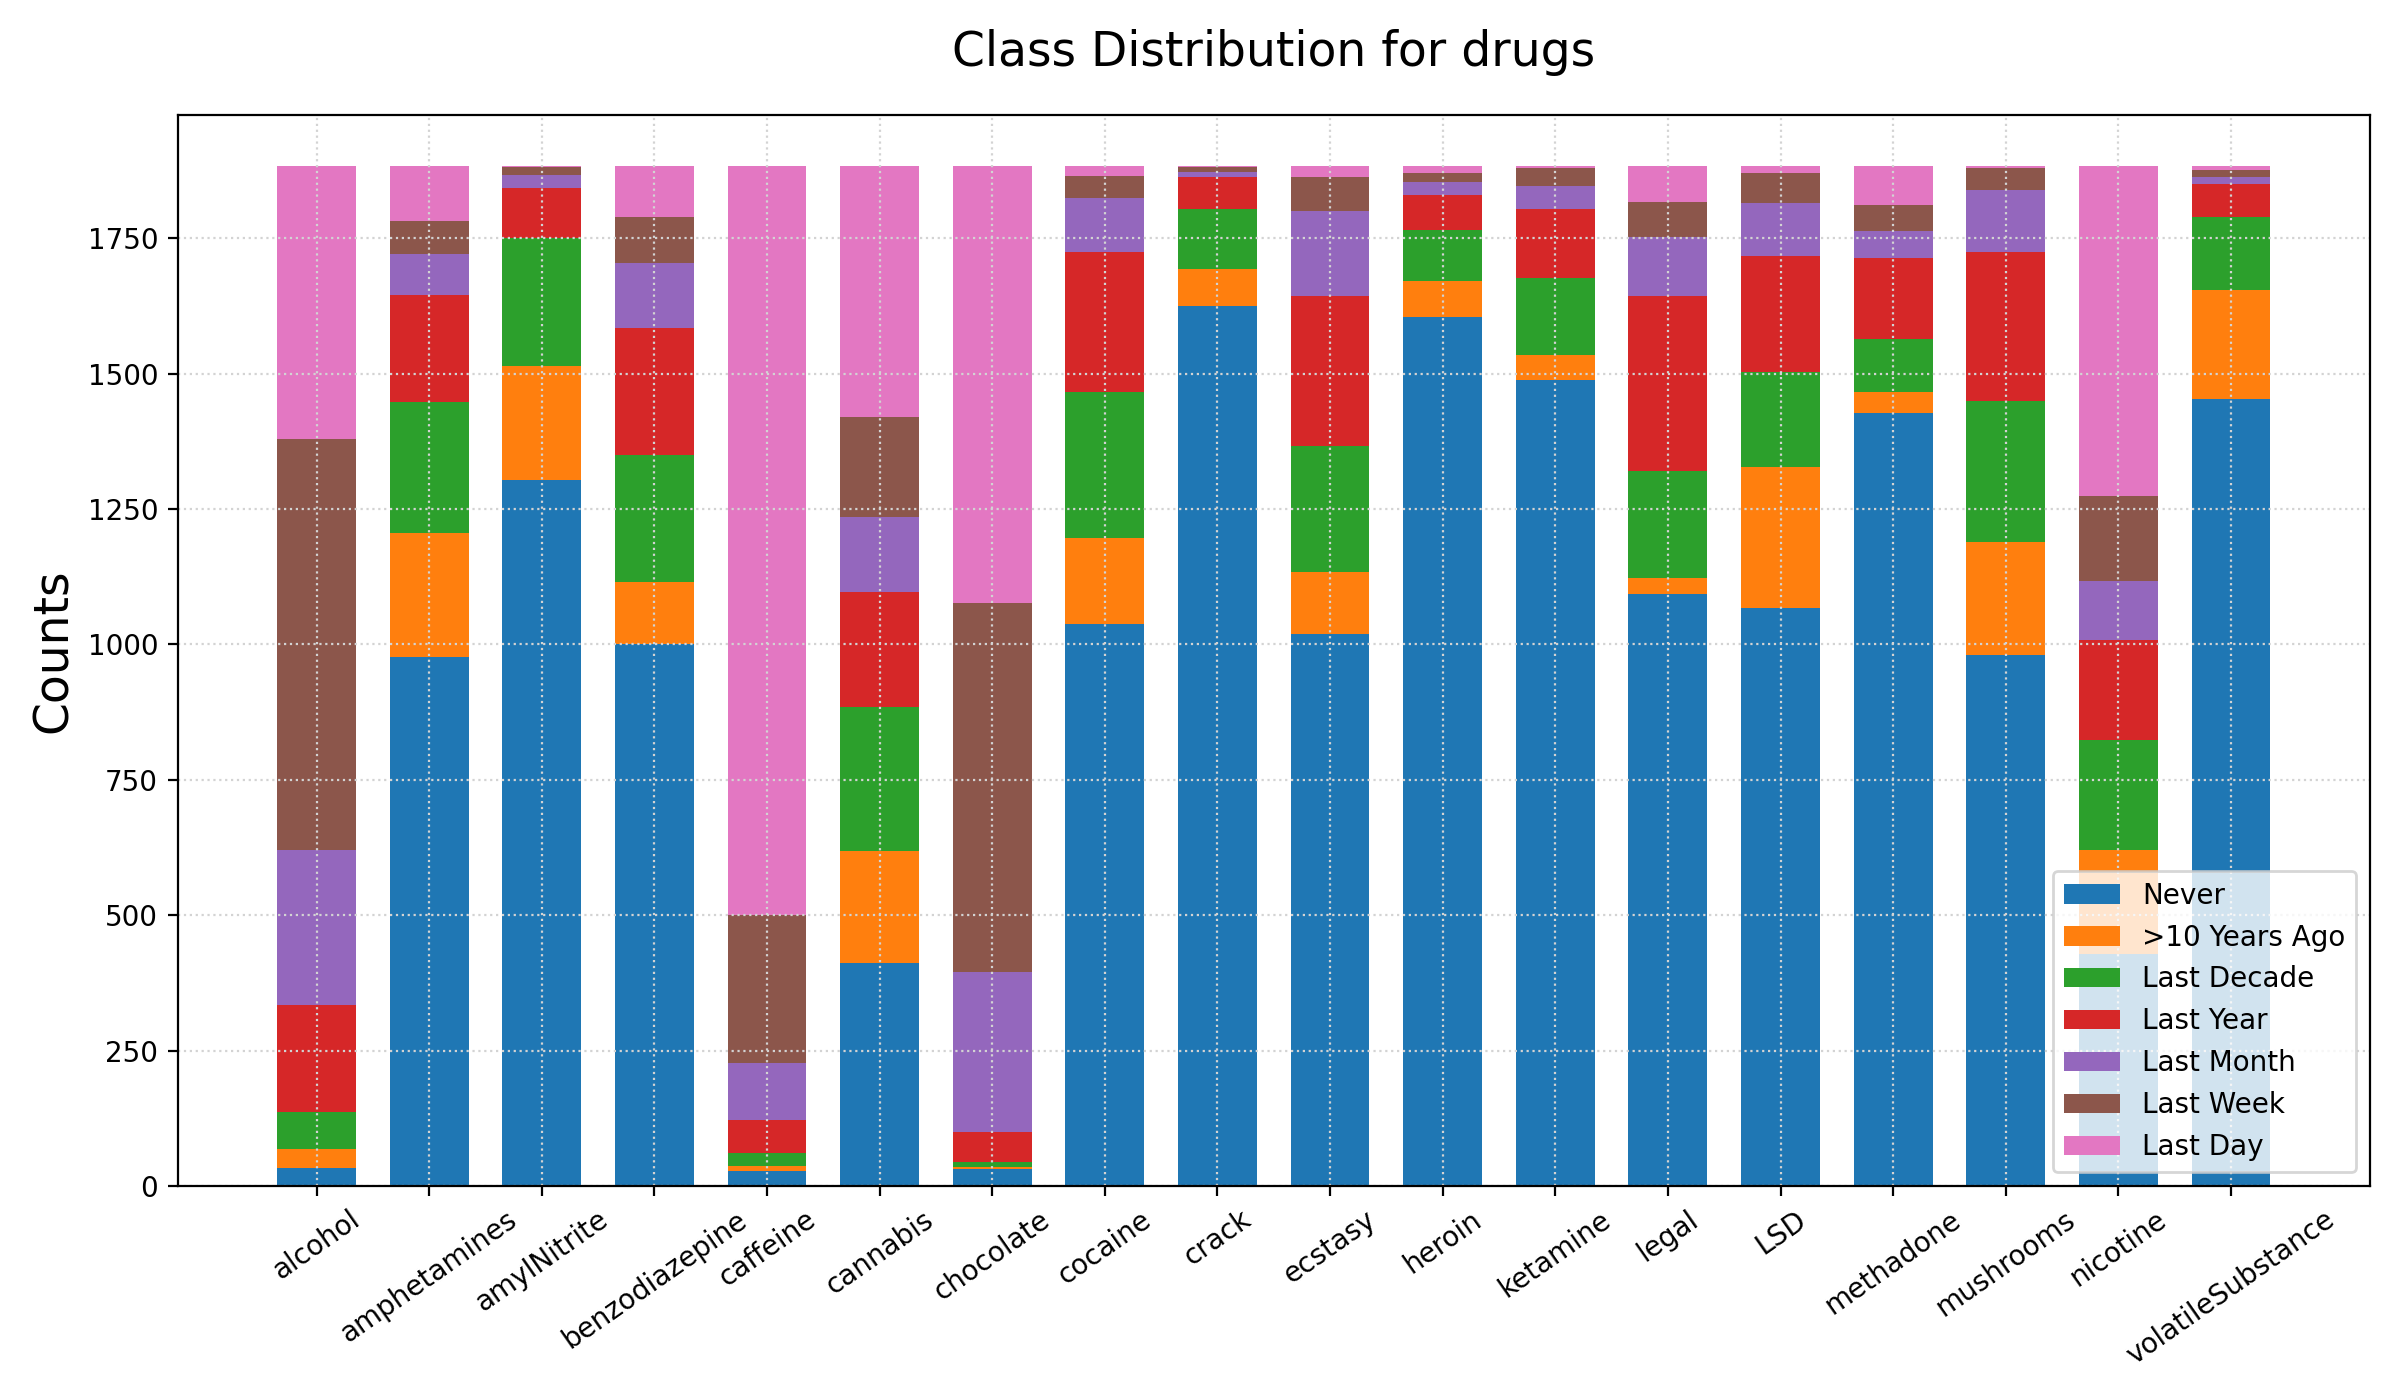
\includegraphics[width=\textwidth]{Plots/Inbalance_drugs.png}
	\end{minipage}
	\begin{minipage}[b]{0.32\textwidth}
	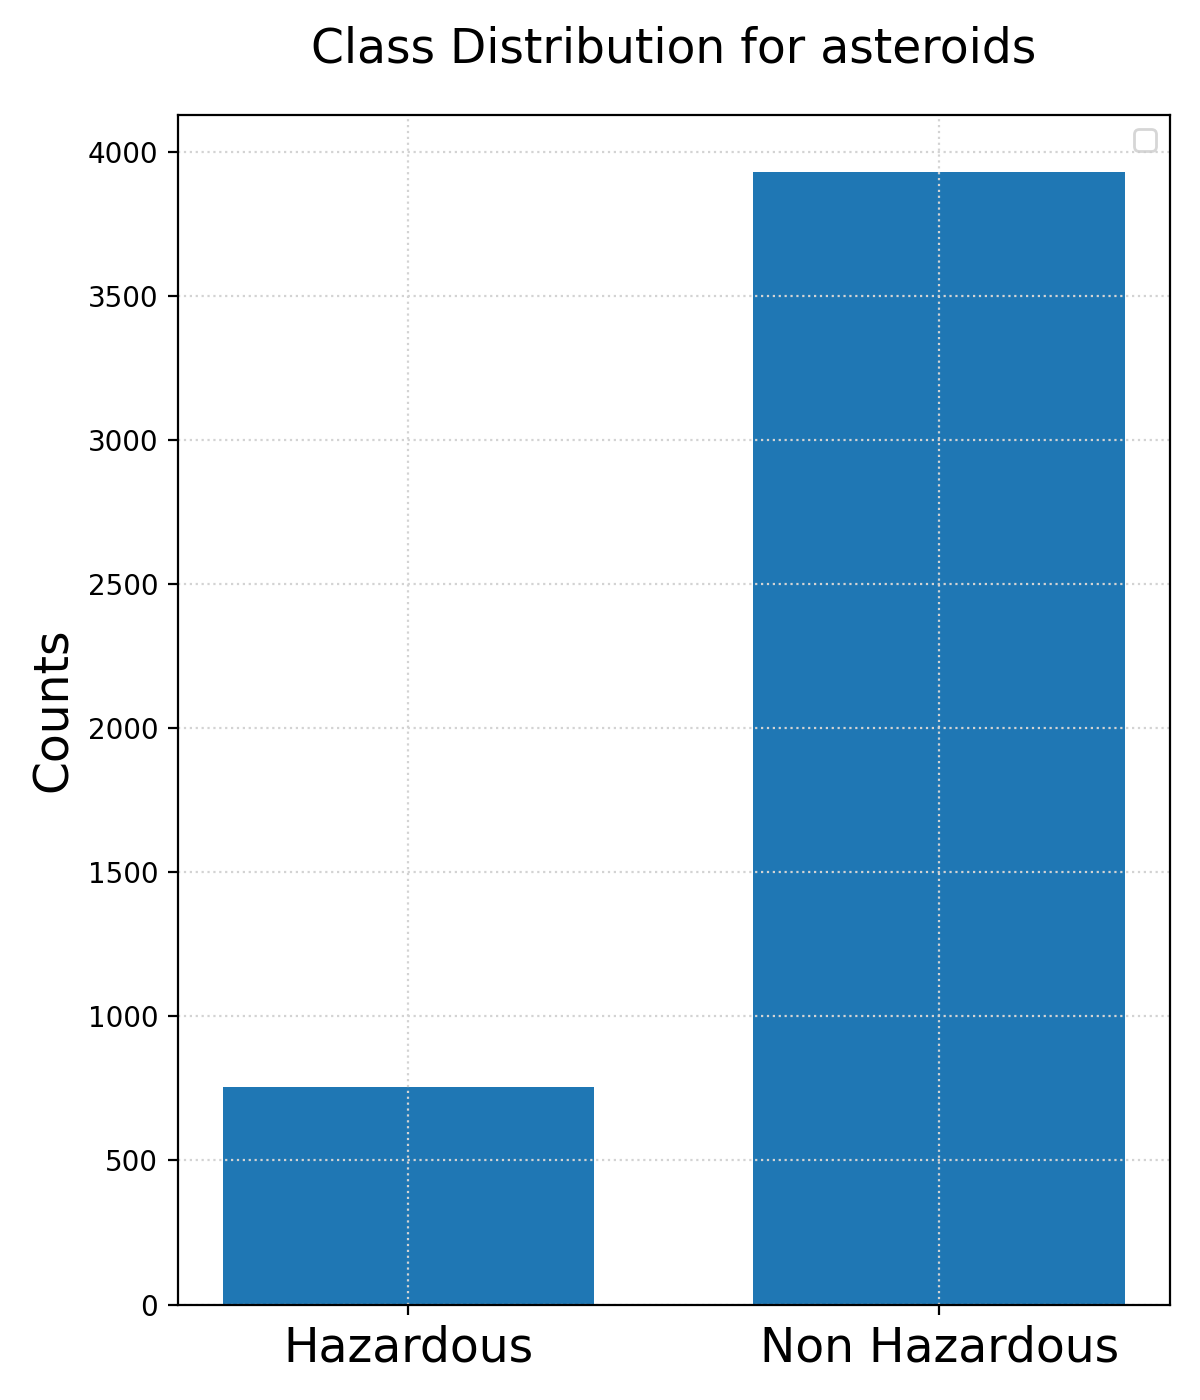
\includegraphics[width=\textwidth]{Plots/Inbalance_asteroids.png}
	\end{minipage}
	\begin{minipage}[b]{0.32\textwidth}
	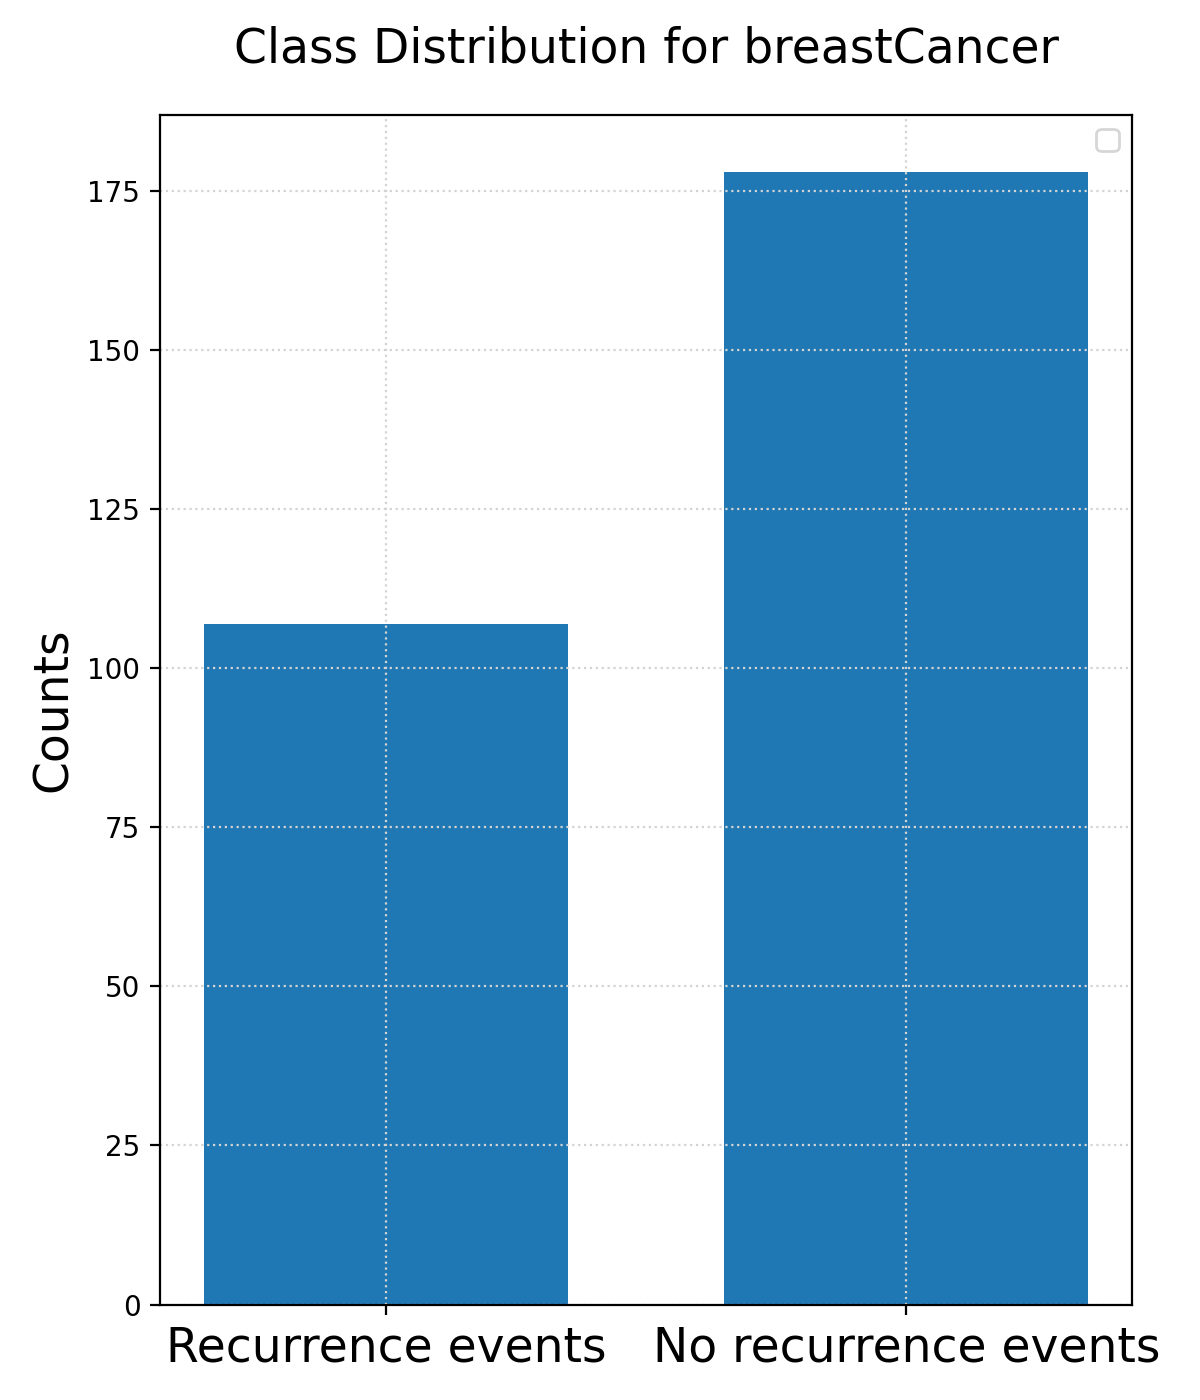
\includegraphics[width=\textwidth]{Plots/Inbalance_breastCancer.png}
	\end{minipage}
	\begin{minipage}[b]{0.32\textwidth}
	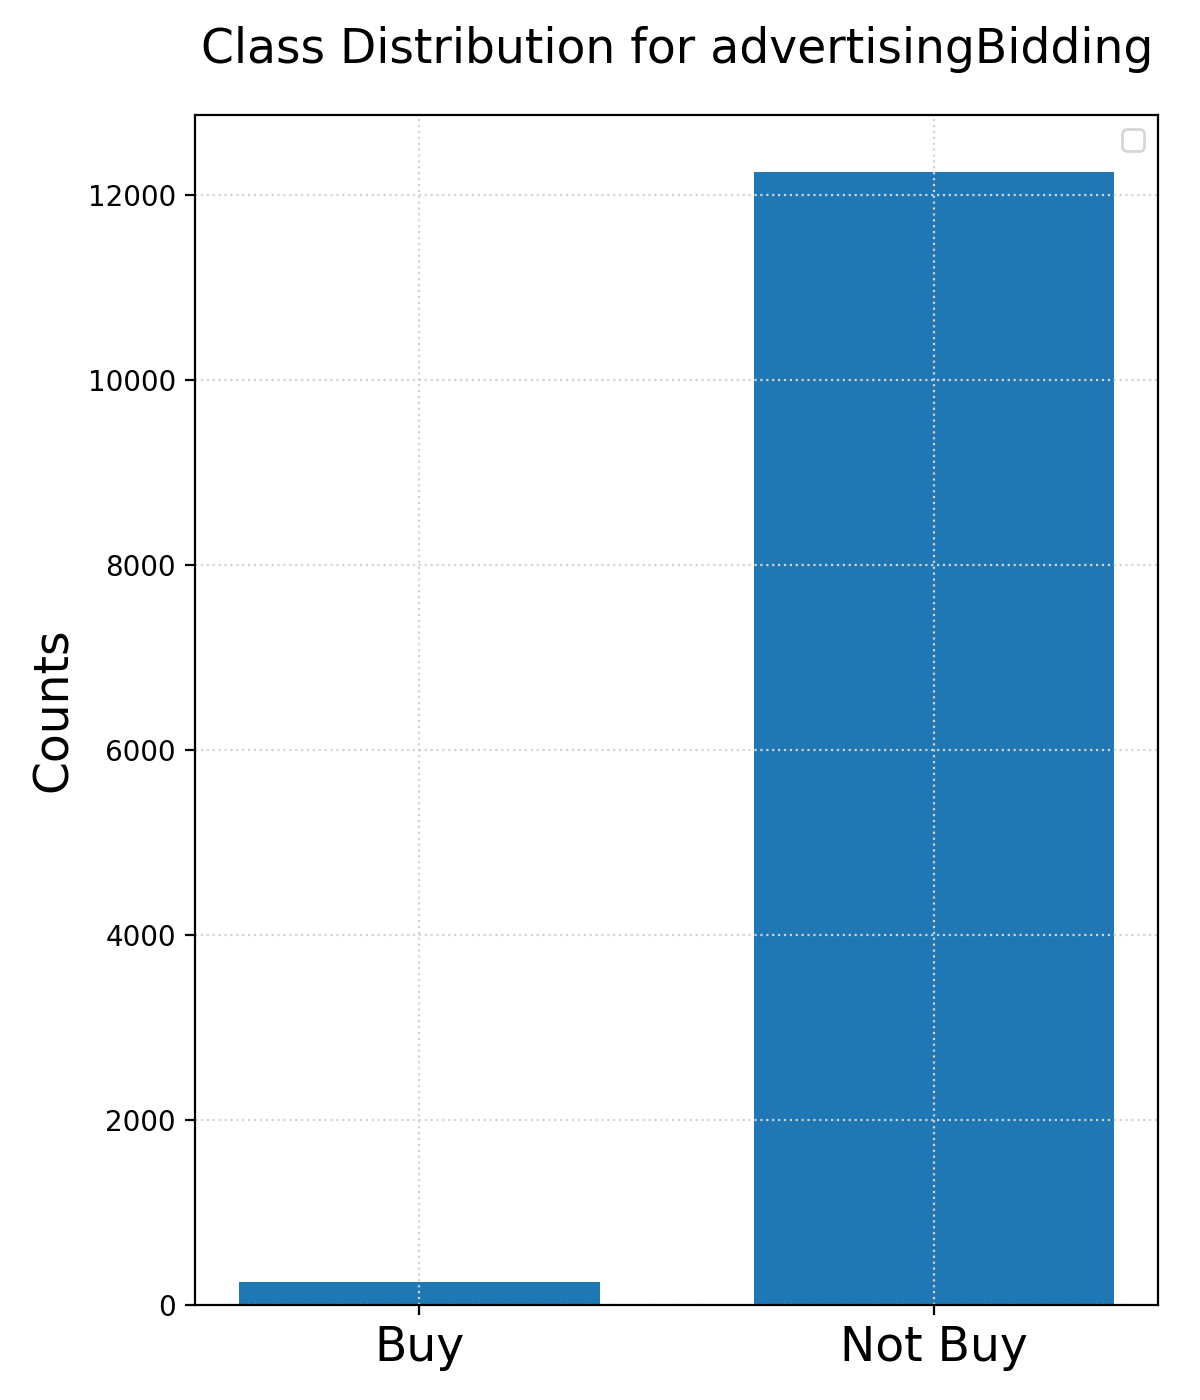
\includegraphics[width=\textwidth]{Plots/Inbalance_advertisingBidding.png}
    \end{minipage}
	\caption{Distribution of classes for the target attributes for the multiclass classification (top panel, drug dataset) and binary classification (bottom panel, asteroids, breast cancer and advertising bidding datasets).}
	\label{fig:imbalance}
\end{figure}

In order to balance the dataset for the binary classification, we implemented and algorithm that performs the following steps.
First, it extracts the number of entries in the under-represented class (which by chance is always class "True" for the three binary classification tasks). Then we randomly select a number of rows from the remaining data of where class is equal to "False", adding an extra $10\%$ to this total. Then, we create a final dataset combining the rows with the class "True" and the randomly selected "False".
This step is done at a preliminary phase before any splitting into the training and testing subsets.


\section{Analysis}
In this section we finally present the results of our classification tasks.

\subsection{Drug consumption}

Overall the performance of the classification is rather insufficient. Looking at the confusion matrices we can see the expected influence of the data imbalance (Fig.\ref{fig:conf_matr_alcohol} App.\ref{app:drug_conf_matr}). The overall fitting strategy is towards the most dominant class whereas the decision tree seems to be the most resistant against this bias when looking at the distribution around the main diagonal. \\

This bias can also influence the performance metrics (P,R,A) - looking at Eqs.\ref{eq:model_training_parameters} one can see that guessing the major class will give values closer and closer to 1 the bigger the imbalance is. This is illustrated in Tab.\ref{tab:accuracy_kNN_selection} where we look at the accuracies under the kNN classifier of a selection of drugs. Together with the class distribution (Fig.\ref{fig:imbalance}) one can observe a positive correlation between the accuracy and the imbalance of the data - this will make it hard to compare drugs to each other using the accuracy as the metric. The influence on the accuracy is also given within the same drug. The kNN classifier shows the same behavior for all drugs, that is, to fixate on the major class(es) with increasing number $k$ of considered neighbors. By comparison of the confusion matrices the kNN classifier isn't only showing this behavior the most out of all classifiers, it also always has the highest accuracy out of all.\\

\begin{figure}[h!]
	\centering
	\begin{minipage}[b]{0.32\textwidth}
		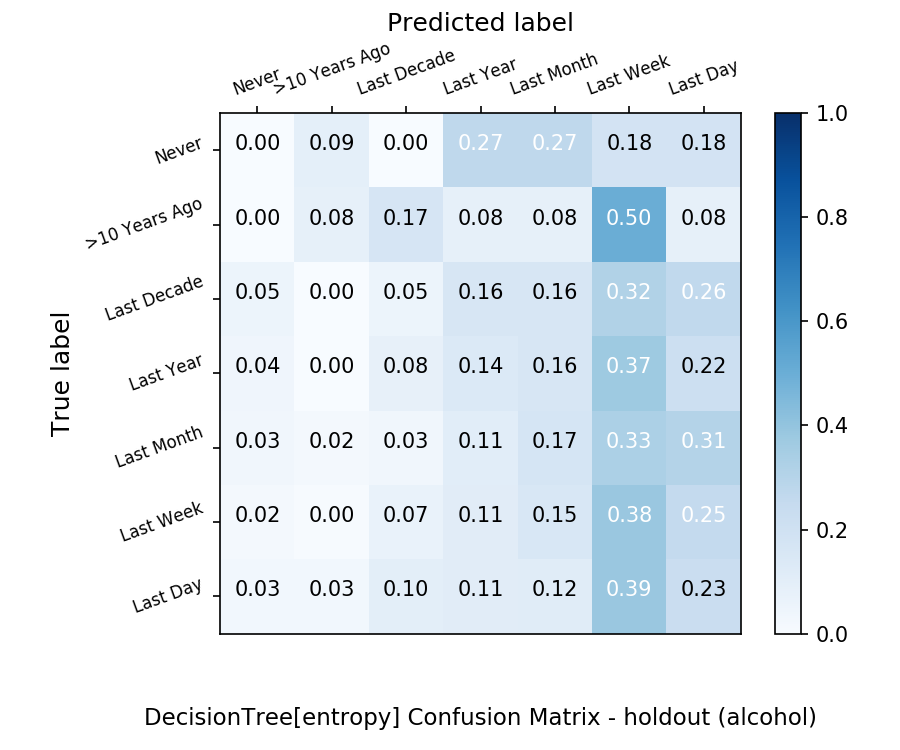
\includegraphics[width=1.1\textwidth]{Plots/drugs/alcohol_DecisionTree_entropy_balance_False_holdout.png}
	\end{minipage}
	\begin{minipage}[b]{0.32\textwidth}
		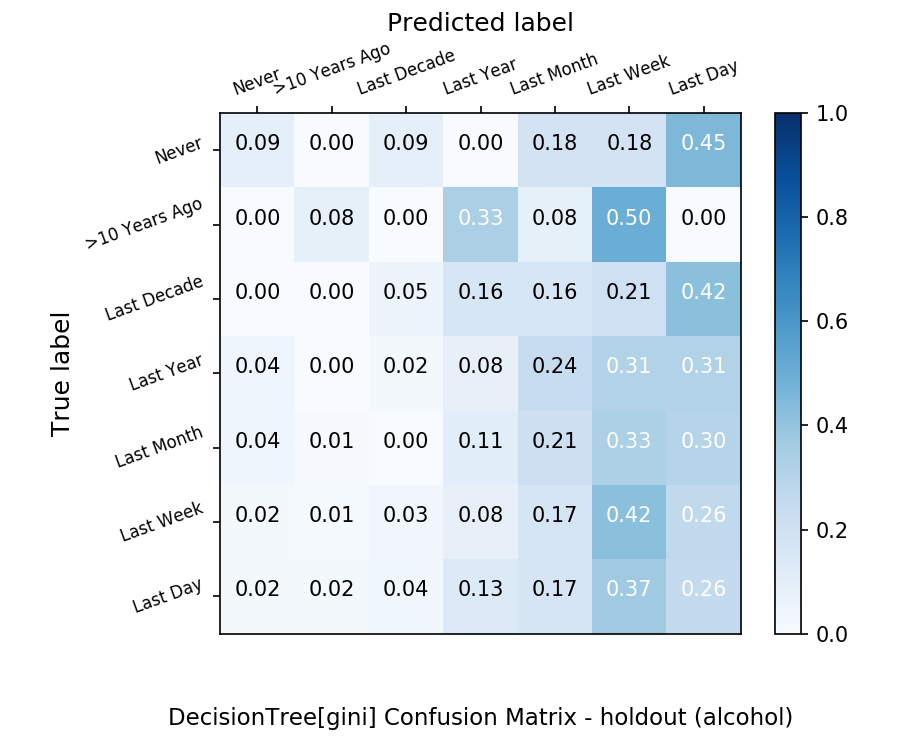
\includegraphics[width=1.1\textwidth]{Plots/drugs/alcohol_DecisionTree_gini_balance_False_holdout.png}
	\end{minipage}
	\begin{minipage}[b]{0.32\textwidth}
		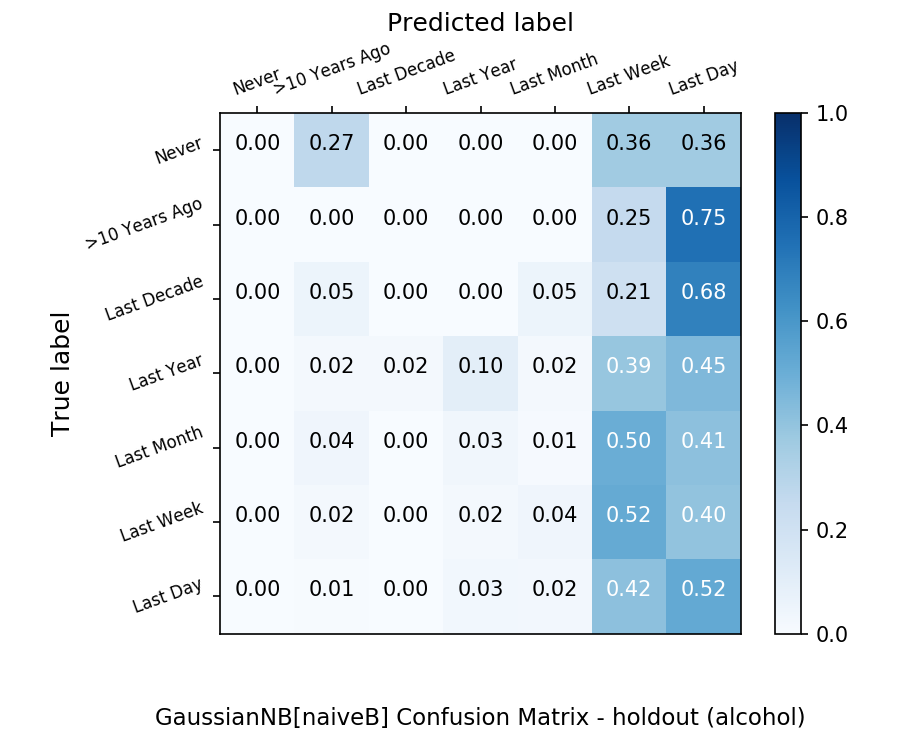
\includegraphics[width=1.1\textwidth]{Plots/drugs/alcohol_GaussianNB_naiveB_balance_False_holdout.png}
	\end{minipage}
	\begin{minipage}[b]{0.32\textwidth}
		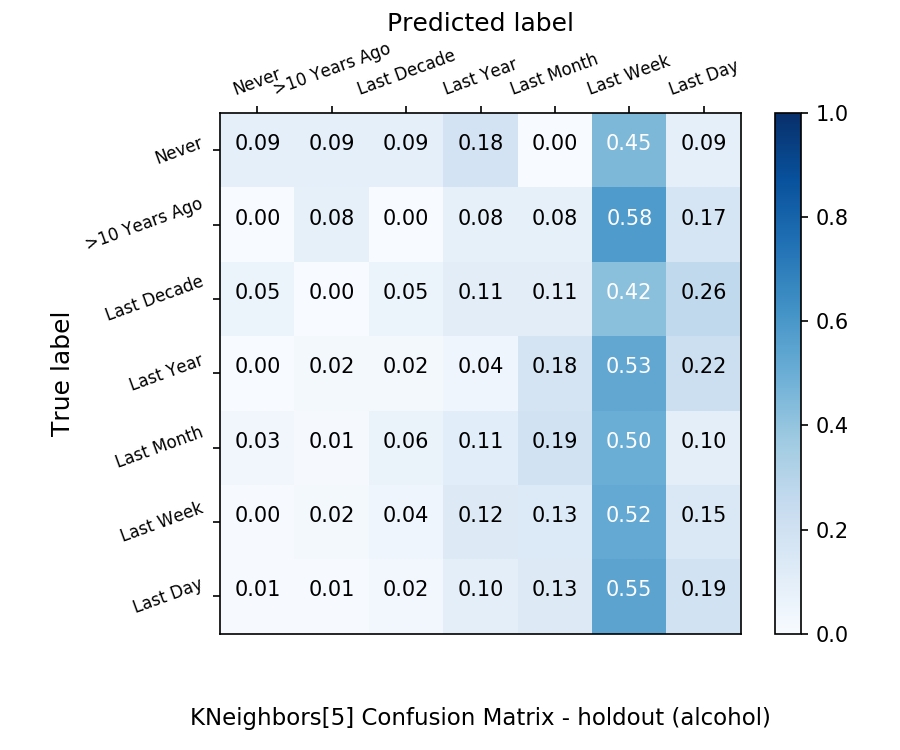
\includegraphics[width=1.1\textwidth]{Plots/drugs/alcohol_KNeighbors_5_balance_False_holdout.png}
  \end{minipage}
	\begin{minipage}[b]{0.32\textwidth}
		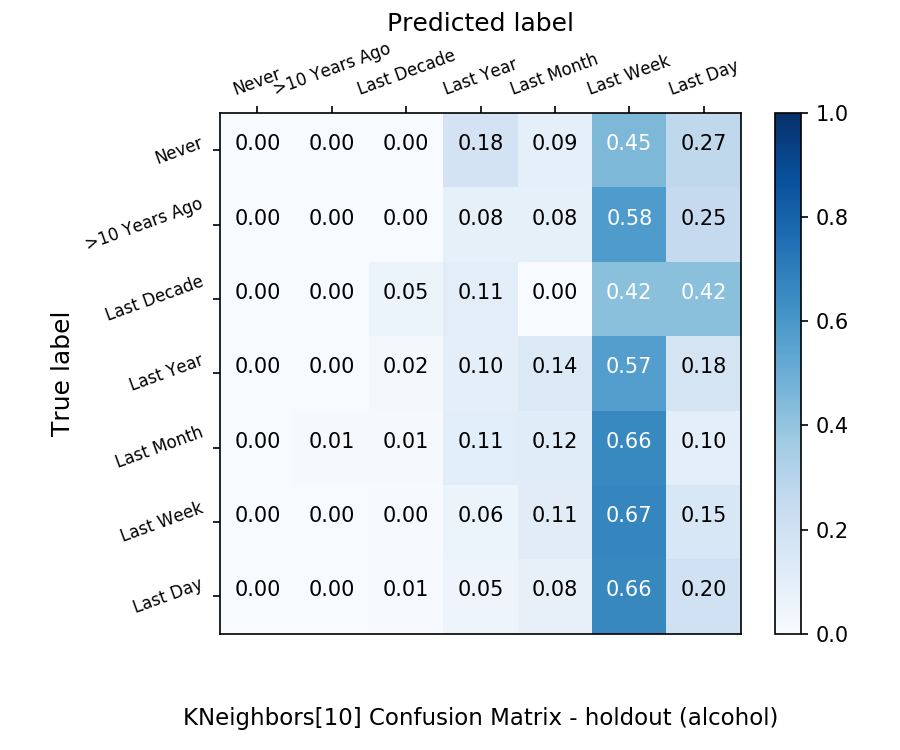
\includegraphics[width=1.1\textwidth]{Plots/drugs/alcohol_KNeighbors_10_balance_False_holdout.png}
  \end{minipage}
	\begin{minipage}[b]{0.32\textwidth}
		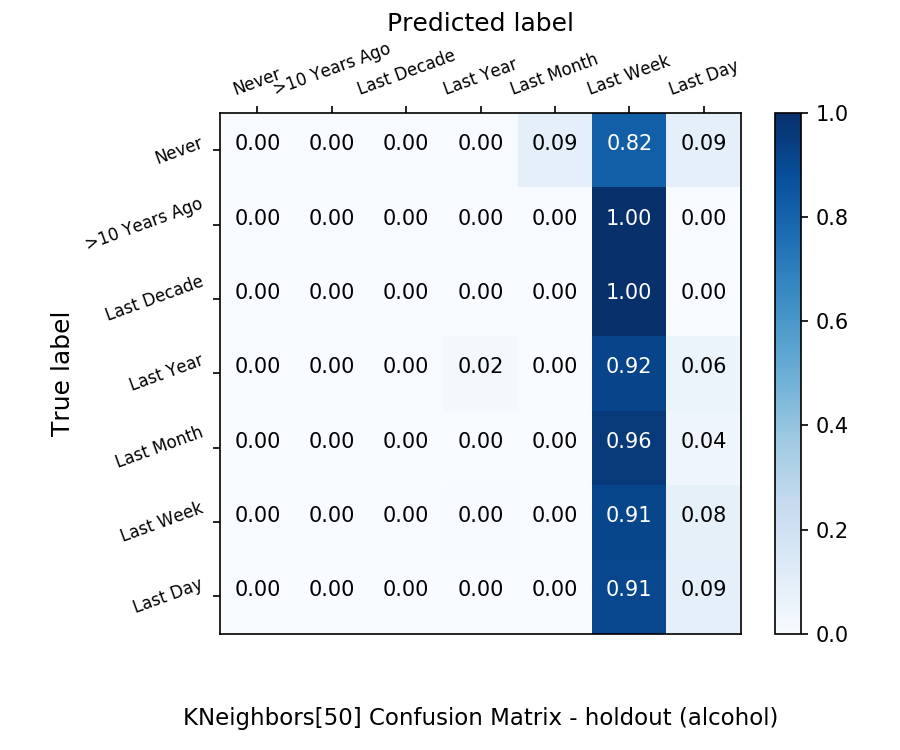
\includegraphics[width=1.1\textwidth]{Plots/drugs/alcohol_KNeighbors_50_balance_False_holdout.png}
  \end{minipage}
	\caption{Confusion matrices for the used classifiers on the drug alcohol.}
	\label{fig:conf_matr_alcohol}
\end{figure}


\begin{table}[h!]
		\centering
    \begin{tabular}{ l c c c }
        \toprule
        \textbf{Drug} & \textbf{k=5 (\%)} & \textbf{k=10 (\%)} & \textbf{k=50 (\%)} \\
        \toprule
        Alcohol & 29.51 & 34.45 & 37.63 \\
        Amyl Nitrite & 66.08 & 68.90 & 70.67 \\
        Cocaine & 49.65 & 54.77 & 56.18 \\
        Methadone & 71.91 & 73.50 & 73.32 \\
        \bottomrule
    \end{tabular}
		\caption{Accuracy of the kNN classifier for the used neighborhood sizes and a selection of drugs.}
		\label{tab:accuracy_kNN_selection}
\end{table}

The remaining metrics in general didn't show any such monotonic behavior. Since the precision and recall were very case-sensitive and an opposing behavior (one high, one low) was observed frequently, we decided to use the $f1$-score as the performance. Tab.\ref{tab:drugs_performance_overview} shows the best performing classifier for each drug and the achieved $f1$-score.
The early assumption that the decision tree is the most resistant and therefore best performing classifier can not be confirmed. Overall we see all classifiers equally represented - the k=50 variant is never best performing and the k=10 only once. In the 4 least imbalanced datasets (alcohol, cannabis, chocolate and nicotine) is no dominant classifier (2x DT, 1x GNB, 1x kNN).

\begin{table}[H]
		\centering
    \begin{tabular}{ l c c c }
        \toprule
        \textbf{Drug} & \textbf{Classifier} & \textbf{$f1$-score} \\
        \toprule
        Alcohol & DT (gini) & 0.172 \\
				Amphetamines & GNB & 0.220 \\
        Amyl Nitrite & GNB & 0.197 \\
				Benzodiazepine & GNB & 0.222 \\
				Caffeine & kNN (k=5) & 0.168 \\
				Cannabis & GNB & 0.246 \\
				Chocolate & DT (entropy) & 0.169 \\
        Cocaine & GNB & 0.219 \\
				Crack & DT (entropy) & 0.236 \\
				Ecstasy & kNN (k=5) & 0.202 \\
				Heroin & kNN (k=5) & 0.181 \\
				Ketamine & DT (gini) & 0.157 \\
				Legal & GNB & 0.233 \\
				LSD & GNB & 0.281 \\
        Methadone & DT (gini) & 0.164 \\
				Mushrooms & kNN (k=10) & 0.264 \\
				Nicotine & kNN (k=5) & 0.204 \\
				Volatile substance & DT (gini) & 0.190 \\
        \bottomrule
    \end{tabular}
		\caption{Best performing classifier for each drug with the achieved $f1$-score.}
		\label{tab:drugs_performance_overview}
\end{table}

As already mentioned, the results aren't good. The imbalance of the data made it hard for the classifiers to find non-trivial patterns in the data and only glimpses could be made. Deeper preprocessing of the data with special attention on single drugs is needed and it could possibly help to drop certain classes, since the drugs can be (apart from few exceptions) split in the two categories "everyday drug" with a big majority in class "Used last day" and the "marginal drugs" with a big majority in "Never used". Focusing on the classes CL1-CL5.


As a final comparison, we show in Fig. \ref{fig:drugs_comparison} the values for the precision and recall for the naive Bayes, the decision trees(Gini) and the kNN(k=10) algorithms. 


\begin{figure}[h!]
	\centering
	\begin{minipage}[b]{0.32\textwidth}
		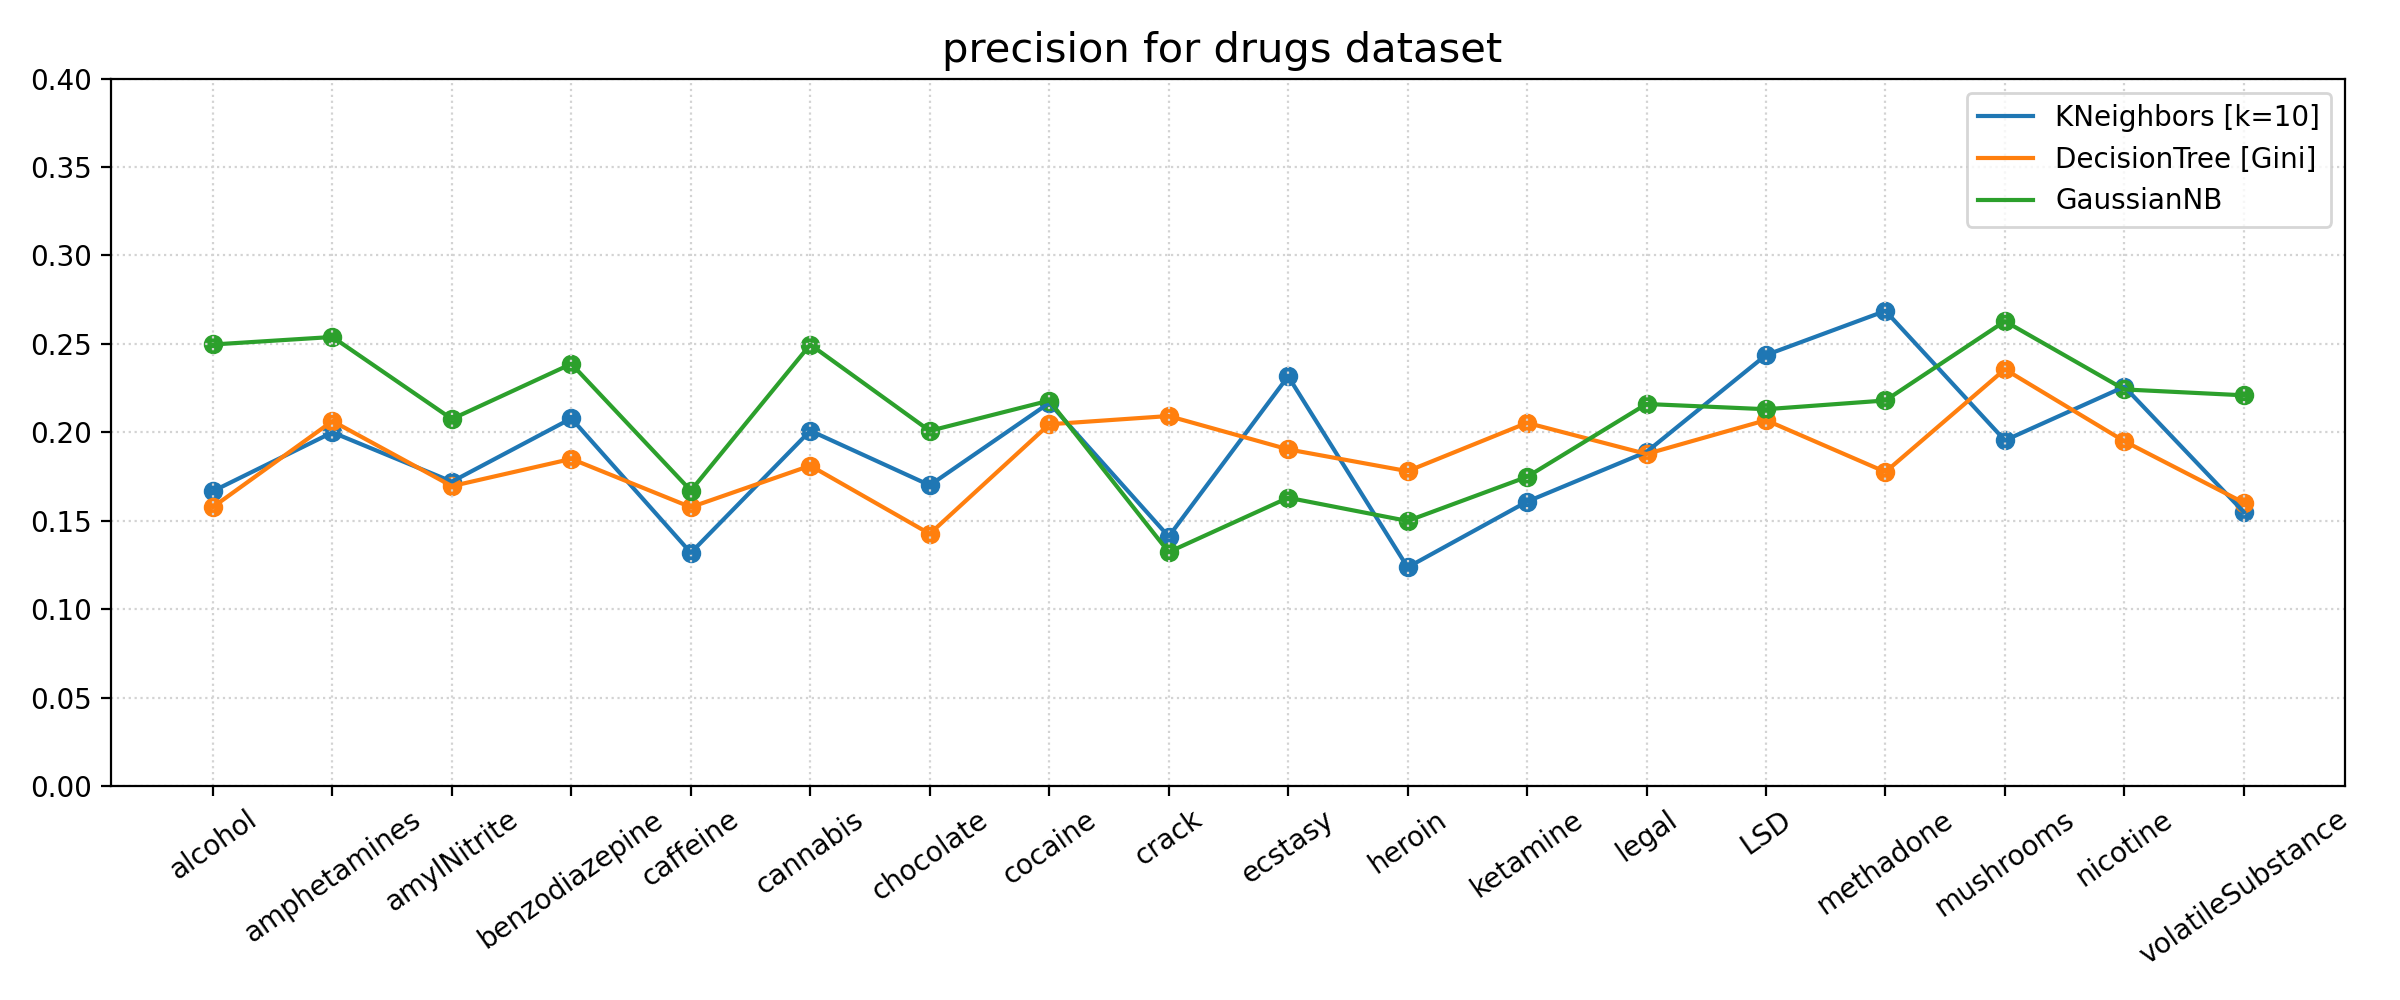
\includegraphics[width=1.1\textwidth]{Plots/precision_comparison_drugs.png}
	\end{minipage}
	\begin{minipage}[b]{0.32\textwidth}
		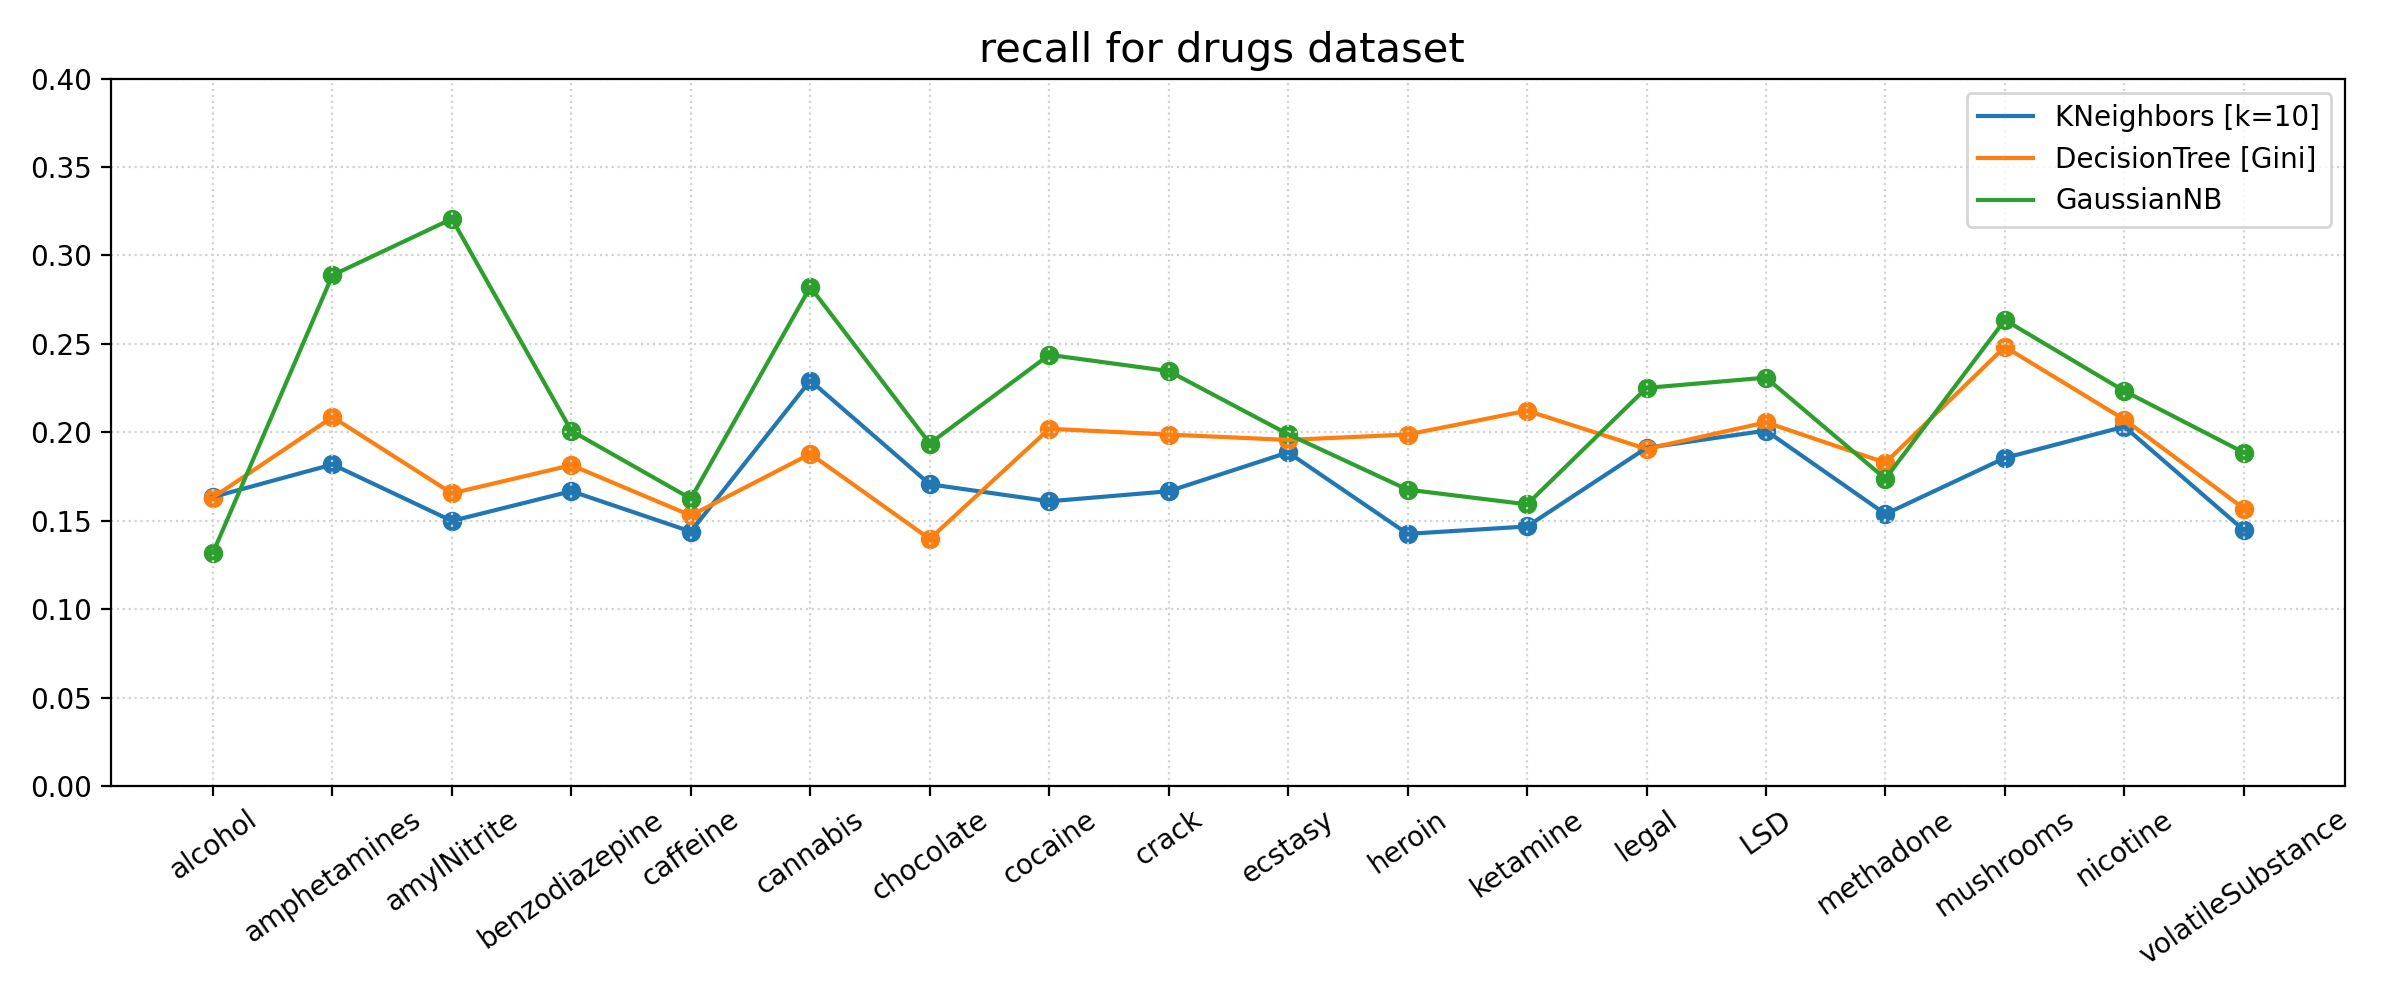
\includegraphics[width=1.1\textwidth]{Plots/recall_comparison_drugs.png}
	\end{minipage}
	\label{fig:drugs_comparison}
\end{figure}








\subsection{Asteroids}

For the asteroids dataset we had 4 comparisons - combinations of balancing (yes/no) and holdout/cross-validation. The comparison on whether to balance the datasets or not, goes in favour of the balanced dataset for the kNN and Gaussian Naive Bayes classifier (see Fig.\ref{fig:conf_matr_asteroids_bal_vs_nonbal} as example) whereas the Decision Tree worked very well in both cases (see below). Holdout and cross-validation dont give a significant improvement over each other. \\

This dataset has a big discrepancy between the classifiers. While both GNB and kNN benefit of reducing the imbalance to avoid a trivial classification, they both don't converge on an acceptable solution. Fig.\ref{fig:conf_matr_asteroids_bal_vs_nonbal} shows how after resampling the best guess seems to be a random one. This is true for all combinations in kNN and GNB - with a single exception for GNB on the balanced dataset with holdout (see appendix \ref{app:asteroids_conf_matr}). \\
This also shows in the performance metrics. With this single exception, accuracy, precision, recall and therefore also $f1$ are apart from small fluctuation the same when looking at the balanced data set (the unbalanced dataset suffers from the same problem as with the drug consumption dataset). For the balanced dataset the metrics for are in the range 0.5-0.55 - the one outlier fluctuates similar to the unbalanced dataset.

\begin{figure}[H]
	\centering
	\begin{subfigure}{.5\textwidth}
		\centering
		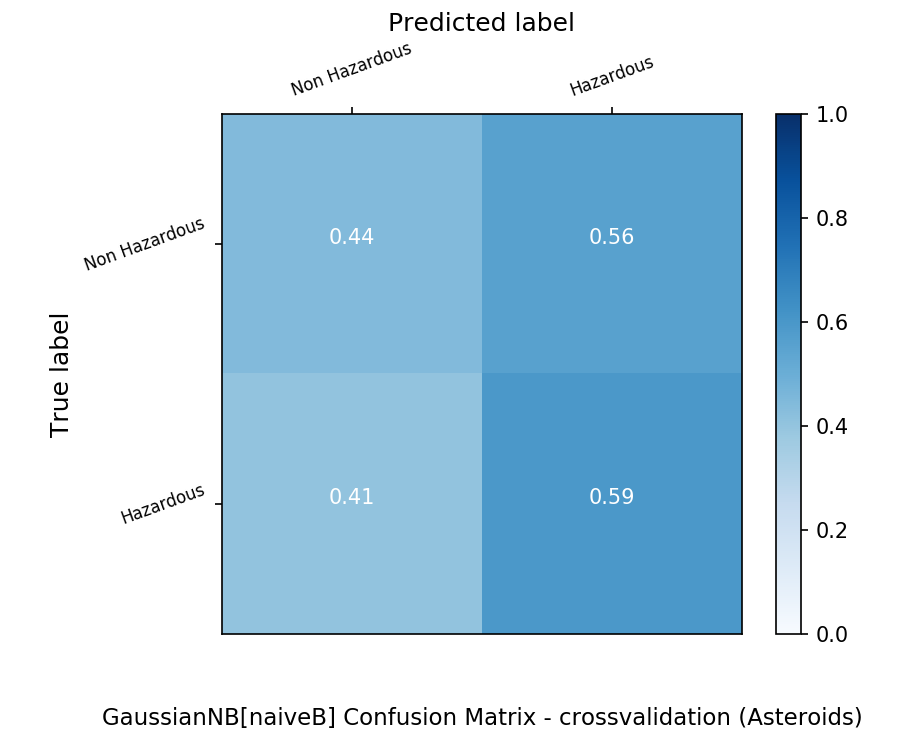
\includegraphics[width=1.1\textwidth]{Plots/asteroids/asteroids_GaussianNB_naiveB_balance_True_crossvalidation.png}
		\caption{balanced}
	\end{subfigure}%
	\begin{subfigure}{.5\textwidth}
		\centering
		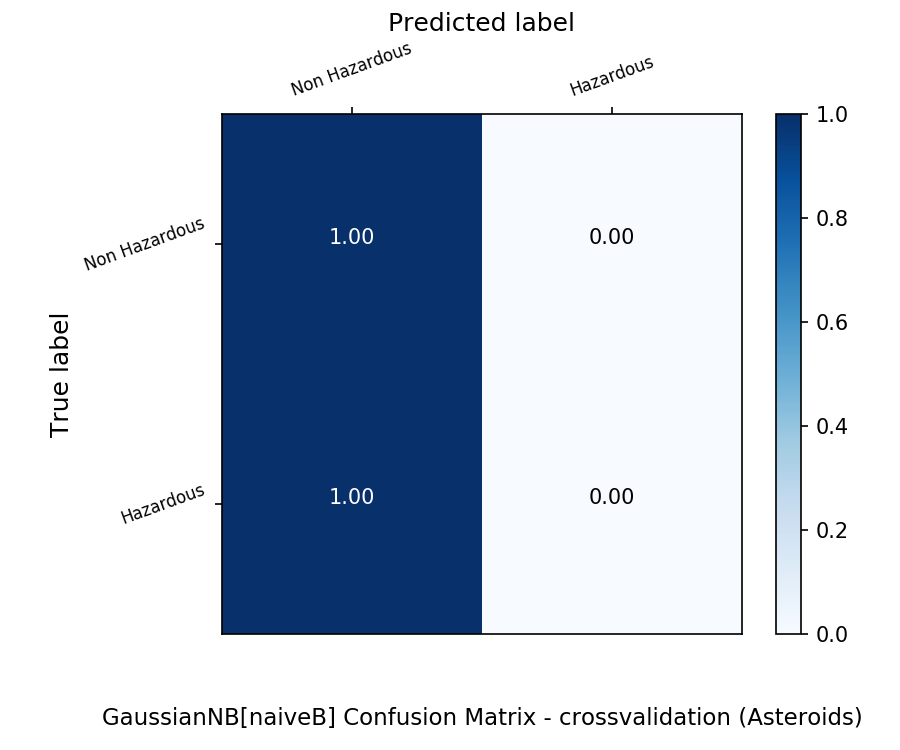
\includegraphics[width=1.1\textwidth]{Plots/asteroids/asteroids_GaussianNB_naiveB_balance_False_crossvalidation.png}
		\caption{non-balanced}
	\end{subfigure}
	\caption{Confusion matrices for the Gaussian Naive Bayes classifier | Effect of balancing the data.}
	\label{fig:conf_matr_asteroids_bal_vs_nonbal}
\end{figure}


Very well performing is the Decision Tree. Not only does it seem to achieve excellent results (Fig.), it also does this independent of the imbalance of the data. Since this result is also achieved with 10-fold cross-validation we are sure that this is not the result of overfitting to the data. With very small fluctuations we achieve scores in the regime of 0.99-1 - the full list can be seen in Tab.\ref{tab:dec_tree_perf_ast}.


\begin{figure}[h!]
	\centering
	\begin{subfigure}{.5\textwidth}
		\centering
		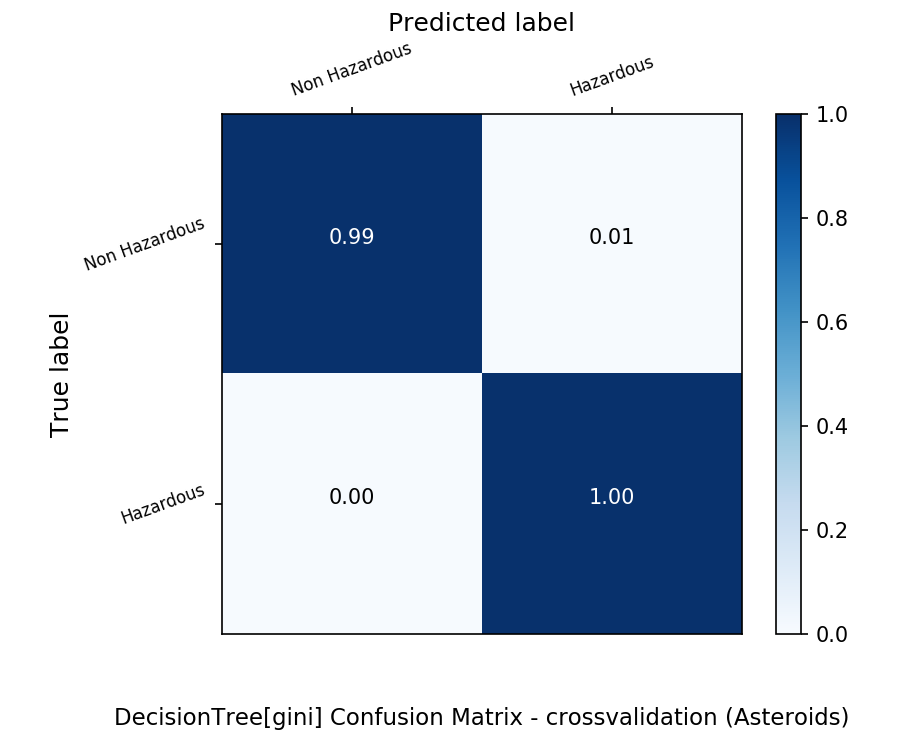
\includegraphics[width=1.1\textwidth]{Plots/asteroids/asteroids_DecisionTree_gini_balance_True_crossvalidation.png}
		\caption{balanced}
	\end{subfigure}%
	\begin{subfigure}{.5\textwidth}
		\centering
		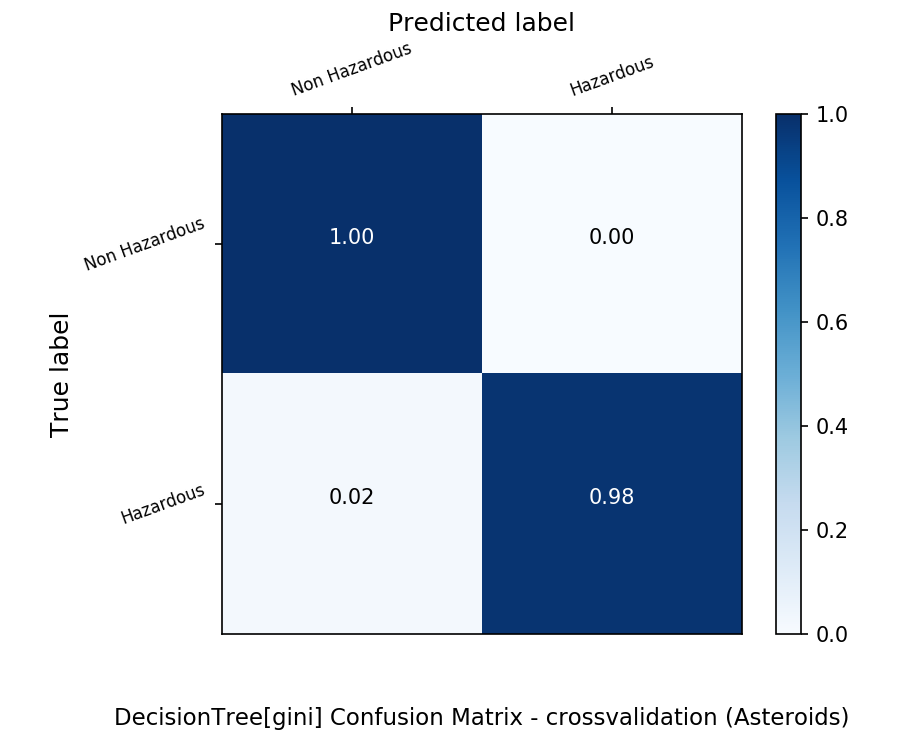
\includegraphics[width=1.1\textwidth]{Plots/asteroids/asteroids_DecisionTree_gini_balance_False_crossvalidation.png}
		\caption{non-balanced}
	\end{subfigure}
	\caption{Confusion matrices for the Decision Tree classifier | Effect of balancing the data.}
	\label{fig:conf_matr_asteroids_bal_vs_nonbal}
\end{figure}

\begin{table}[h!]
		\centering
    \begin{tabular}{ l l l c }
        \toprule
        \textbf{Classfier} & \textbf{Balanced} & \textbf{validation} & \textbf{$f1$-score} \\
        \toprule
        DT (gini) & true & holdout & 0.989 \\
				DT (gini) & true & cv & 0.994 \\
        DT (gini) & false & holdout & 0.992 \\
				DT (gini) & false & cv & 0.994 \\
				DT (entropy) & true & holdout & 0.987 \\
				DT (entropy) & true & cv & 0.993 \\
				DT (entropy) & false & holdout & 0.993 \\
        DT (entropy) & false & cv & 0.993 \\
        \bottomrule
    \end{tabular}
		\caption{$f1$-scores for all Decision Tree combinations.}
		\label{tab:dec_tree_perf_ast}
\end{table}

Understanding the origin of the classification (e.g. all asteroids within close proximity and above a certain size) of the dataset could give some insight on why the Decision Tree is performing so well. It is not clear to us why the other classification algorithms underperform compared to the Decision Tree. One could invest more time to check which features are relevant and which can be dropped - this may also help improving the other classifiers. Nice about this dataset was the illustration of the balancing through under-sampling. This is a step that is definitely needed for GNB and kNN to perform good, even with a reduced feature set.


\subsection{Online advertisement bidding}

\paragraph{kNN algorithm }

If we apply the kNN algorithm in order to classify the online advertisement bidding without balancing the data we obtain a clear case of overfitting.
No matter what parameter we use or if we do holdout or cross validation every instance is placed in the majority class.


\begin{figure}[H]
	\centering
	\begin{subfigure}{.5\textwidth}
		\centering
		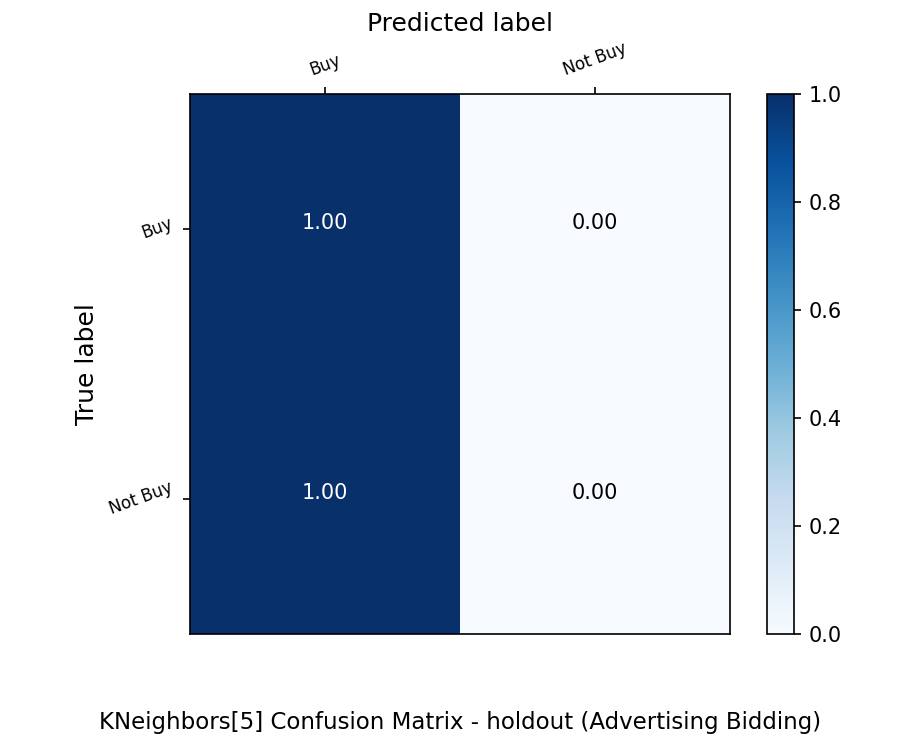
\includegraphics[width=1.1\textwidth]{Plots/conv_KNeighbors_5_balance_False_holdout.png}
		\caption{balanced}
	\end{subfigure}%
	\begin{subfigure}{.5\textwidth}
		\centering
		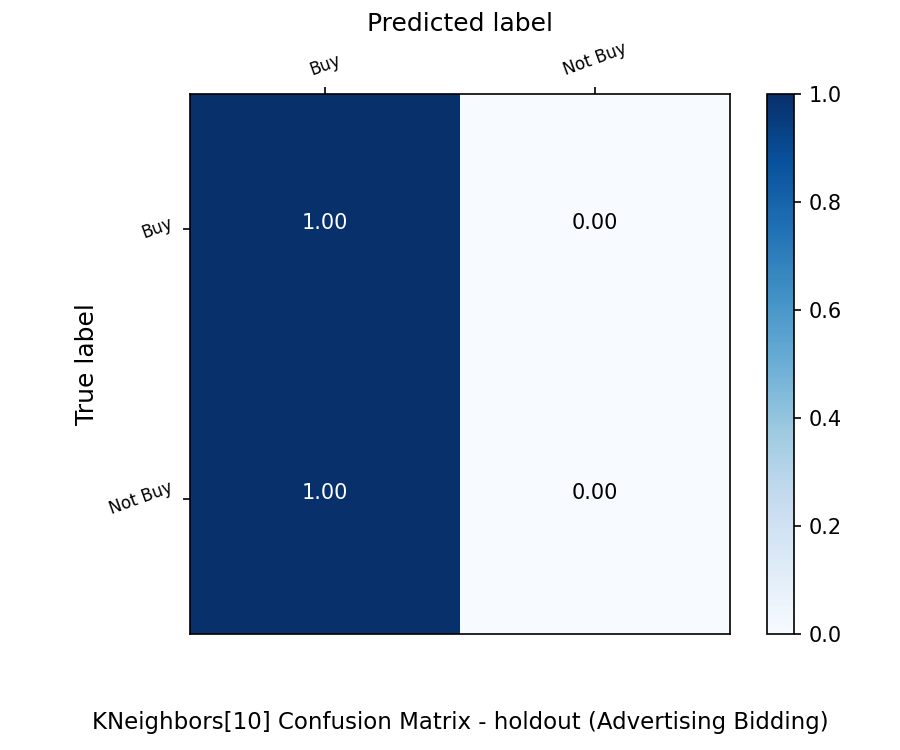
\includegraphics[width=1.1\textwidth]{Plots/conv_KNeighbors_10_balance_False_holdout.png}
		\caption{non-balanced}
	\end{subfigure}
	\caption{{\color{red} Examples of non balanced datasets.}}
\end{figure}


In order to use the classifier we have used k equal to 5, 10 and 50.
From the experiment we can notice that with cross validation the best accuracy is obtained using k=10 (It is close to the 62\% while with k=5 or k=50 it is slightly lower)


\begin{figure}[H]
	\centering
	\begin{subfigure}{.5\textwidth}
		\centering
		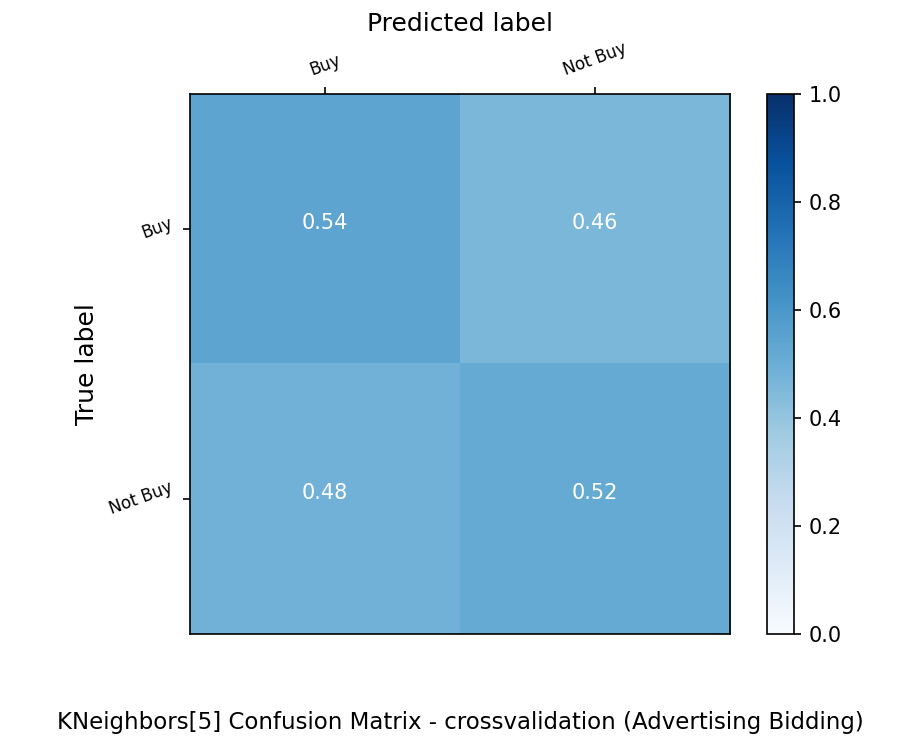
\includegraphics[width=1.1\textwidth]{Plots/conv_KNeighbors_5_balance_True_crossvalidation}
		\caption{balanced}
	\end{subfigure}%
	\begin{subfigure}{.5\textwidth}
		\centering
		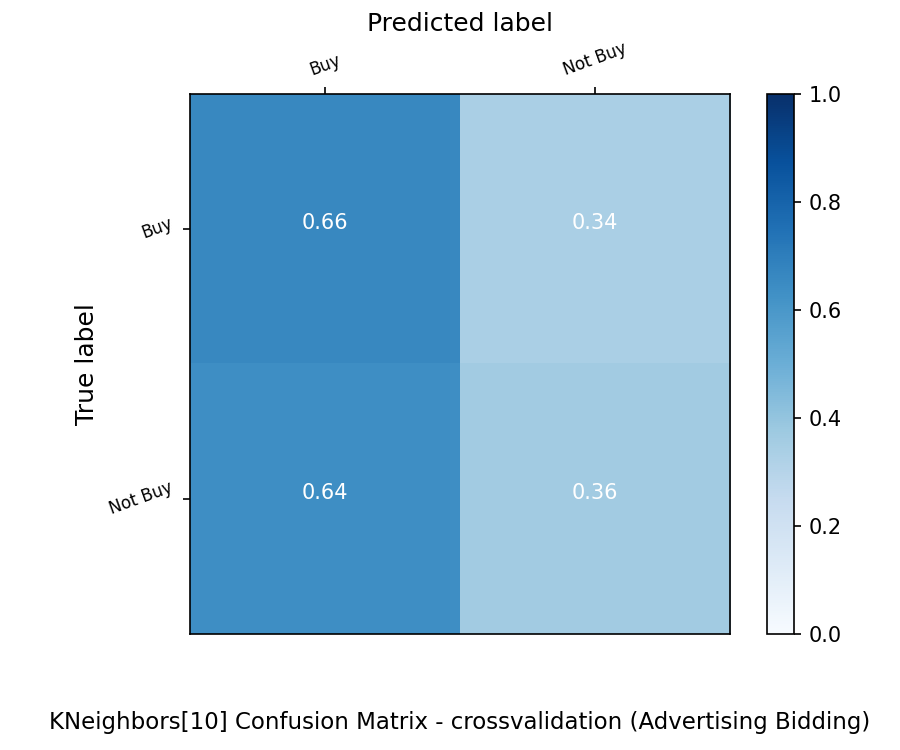
\includegraphics[width=1.1\textwidth]{Plots/conv_KNeighbors_10_balance_True_crossvalidation}
		\caption{non-balanced}
	\end{subfigure}
	\begin{subfigure}{.5\textwidth}
		\centering
		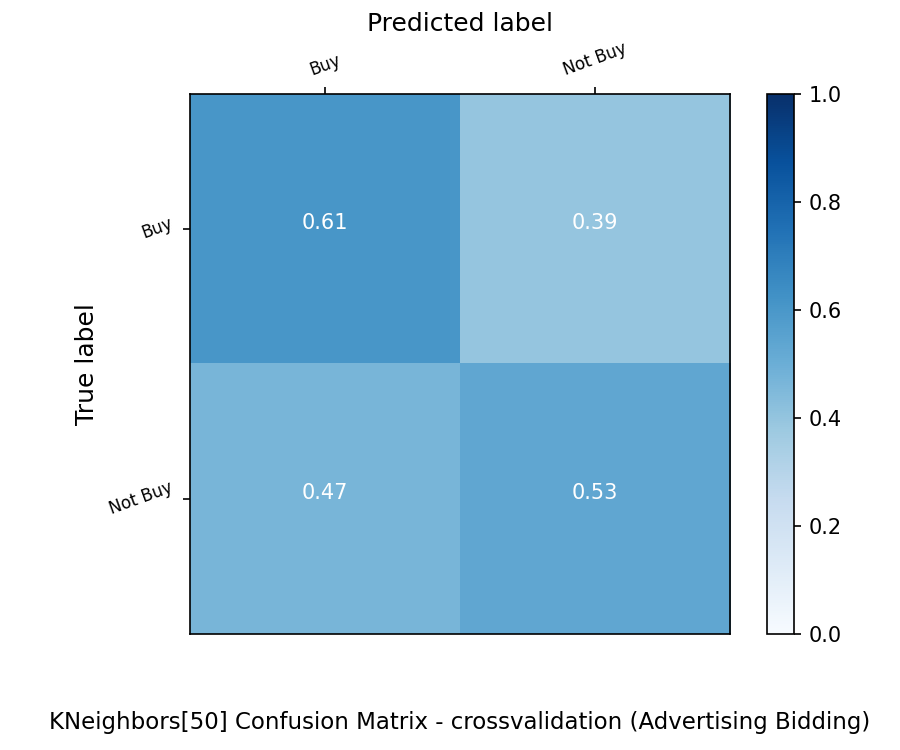
\includegraphics[width=1.1\textwidth]{Plots/conv_KNeighbors_50_balance_True_crossvalidation}
		\caption{non-balanced}
	\end{subfigure}
	\caption{{\color{red}NKK with Cross validation for k=5;10;50}}
\end{figure}


With holdout the best result is  obtained with  k=10 too in fact we have an accuracy of the 66\% while the k=5 and k=50 have accuracy of the 65\% and 64\% respectively.
If we look at precision and recall we have for k=10 66\% and 65\% respectively while for k=5 and k=10 we have lower values.


\begin{figure}[H]
	\centering
	\begin{subfigure}{.5\textwidth}
		\centering
		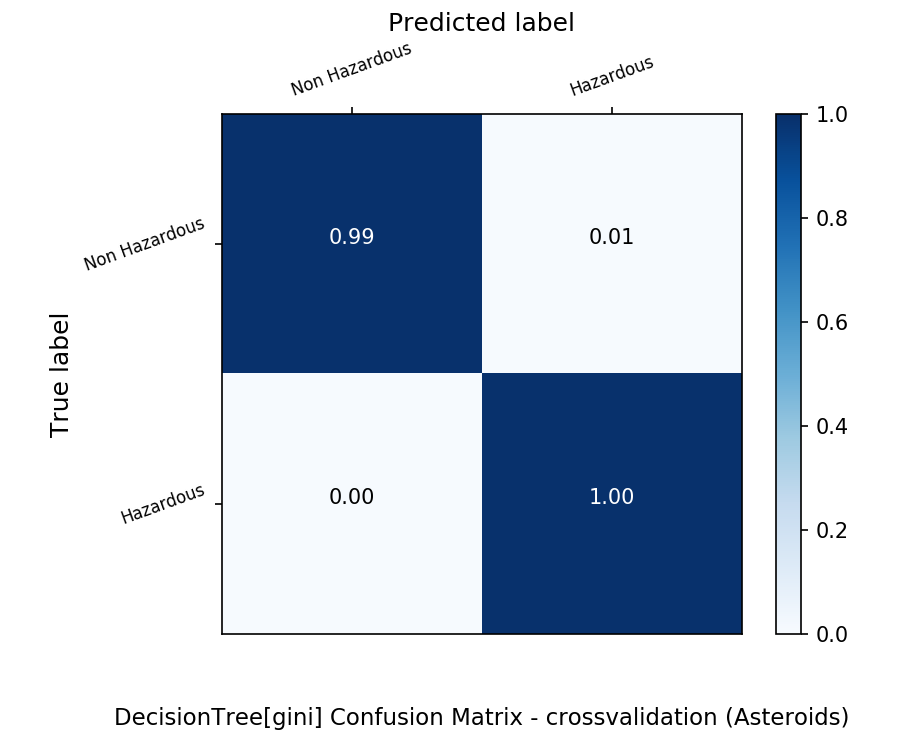
\includegraphics[width=1.1\textwidth]{Plots/asteroids/asteroids_DecisionTree_gini_balance_True_crossvalidation.png}
		\caption{balanced}
	\end{subfigure}%
	\begin{subfigure}{.5\textwidth}
		\centering
		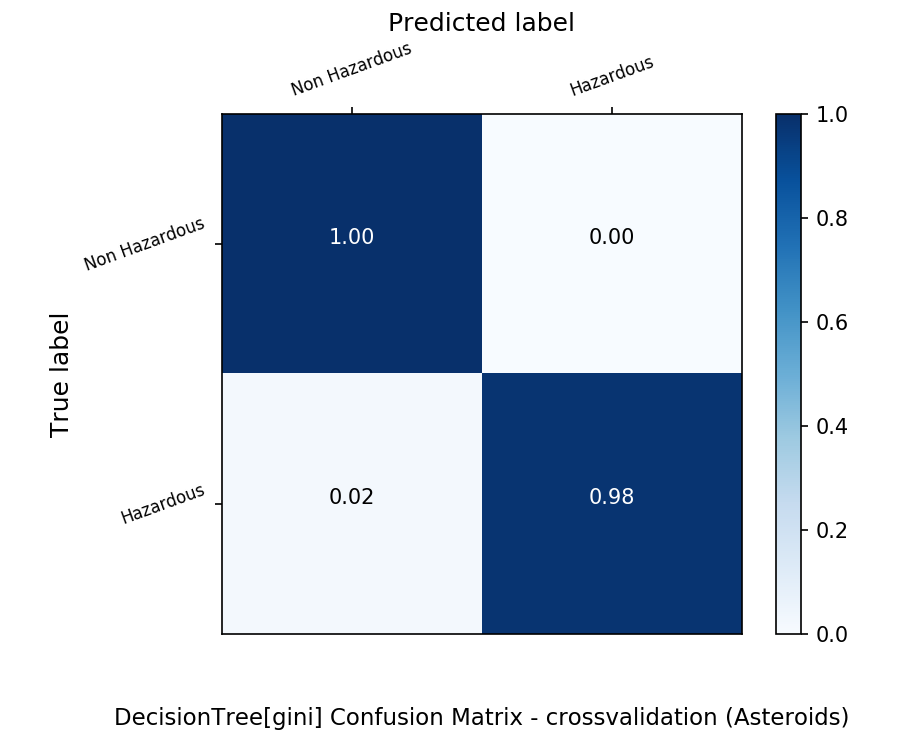
\includegraphics[width=1.1\textwidth]{Plots/asteroids/asteroids_DecisionTree_gini_balance_False_crossvalidation.png}
		\caption{non-balanced}
	\end{subfigure}
	\caption{{\color{red} PLACEHOLDER IMAGES. NEED TO BE CHANGED.}}
\end{figure}


\paragraph{Decision Tree}
If we build the decision tree we can see that from our experiment we get very good results
In fact using the entropy for both cross validation and holdout we get Accuracy, precision and recall equal to 1.
The same results are obtained using the Gini index.


\begin{figure}[H]
	\centering
	\begin{subfigure}{.5\textwidth}
		\centering
		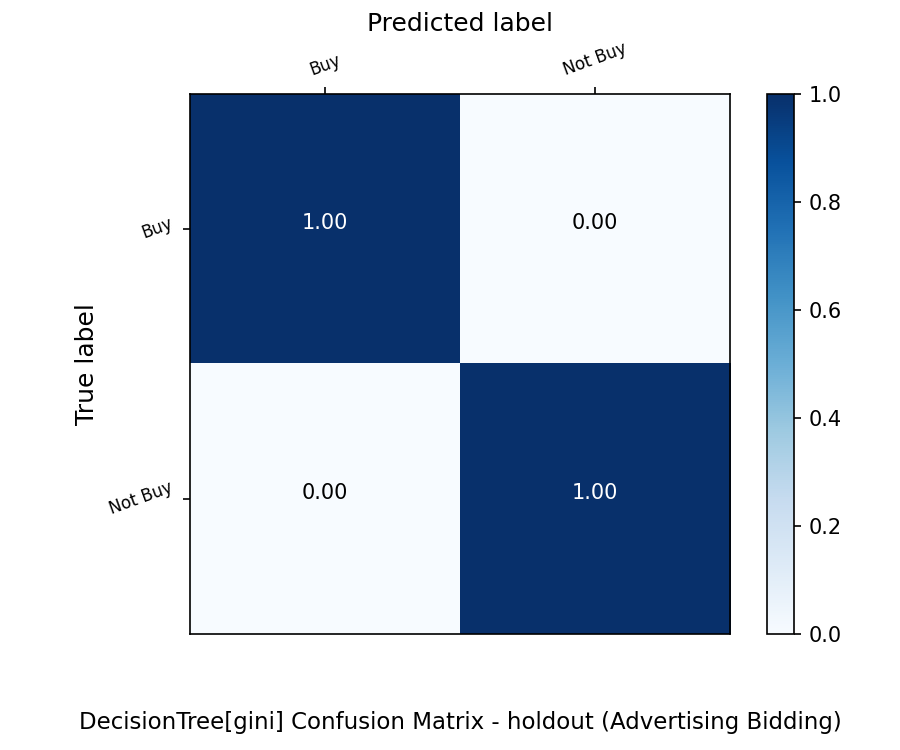
\includegraphics[width=1.1\textwidth]{Plots/advertisingBidding_DecisionTree_gini_balance_True_holdout.png}
		\caption{balanced}
	\end{subfigure}%
	\begin{subfigure}{.5\textwidth}
		\centering
		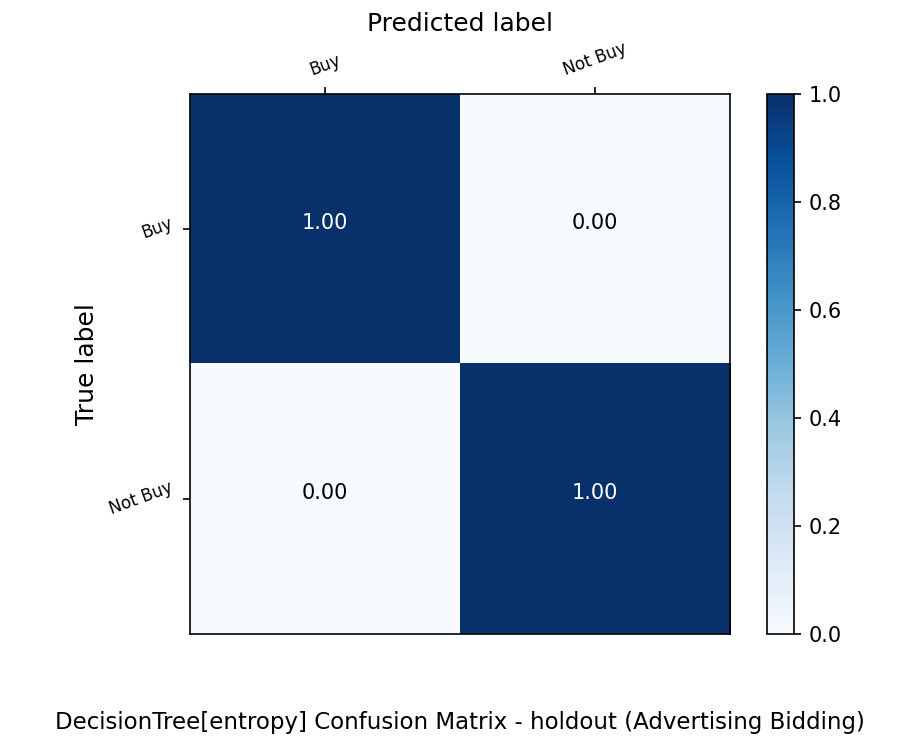
\includegraphics[width=1.1\textwidth]{Plots/advertisingBidding_DecisionTree_entropy_balance_True_holdout.png}
		\caption{non-balanced}
	\end{subfigure}
	\caption{{\color{red} Decision trees using Gini index and Entropy}}
\end{figure}


\paragraph{Naive Bayes}
Also with naive Bayes we get very good results in fact as for the decision tree the accuracy the precision and the recall are 1.


\begin{figure}[H]
	\centering
	\begin{subfigure}{.5\textwidth}
		\centering
		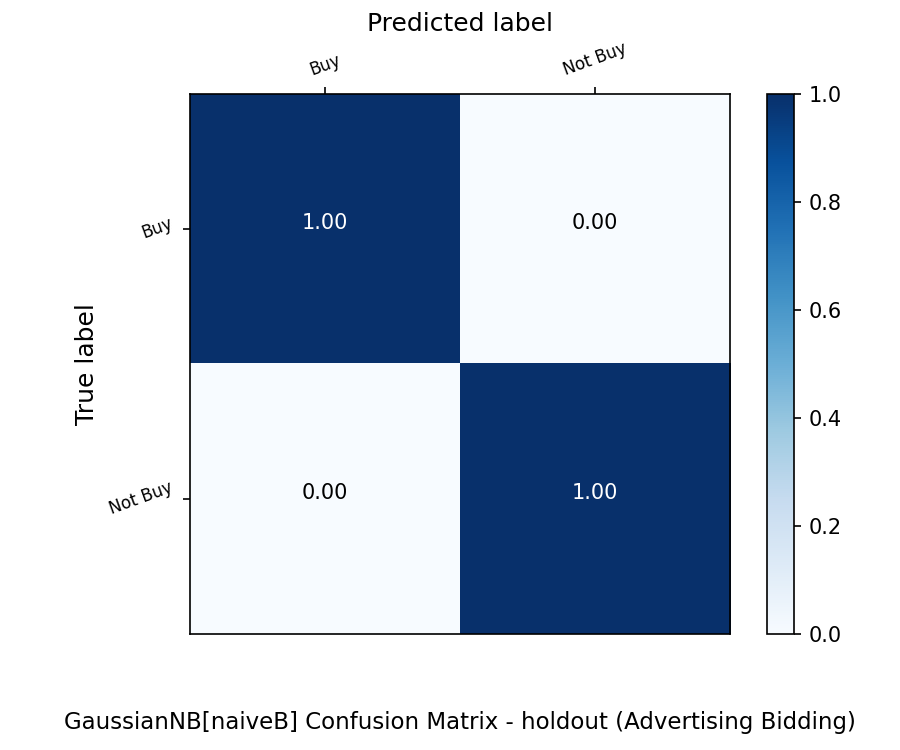
\includegraphics[width=1.1\textwidth]{Plots/advertisingBidding_GaussianNB_naiveB_balance_True_holdout.png}
		\caption{balanced}
	\end{subfigure}%
	\caption{{\color{red} Naive Bayes classifier result.}}
\end{figure}


Looking at the experiment results we can notice that for the Online bidding advertisement the decision tree classifier and the Naive Bayes classifier produce better results than the KNN classifier.





\subsection{Breast cancer}


\paragraph{kNN algorithm }

Considering the hold out balanced data for k=5 we get the values shown in Tab.\ref{tab:perf_kNN_breast}. Using cross-validation increases this values to A=95\%, P=95\% and R=94\% for k=5 and roughly 100\% for k=10 and k=50. \\
For the kNN classifier the results turn out to be the best for k=10.

\begin{table}[h!]
		\centering
    \begin{tabular}{ l c c c }
        \toprule
        \textbf{k} & \textbf{Accuracy (\%)} & \textbf{Precision (\%)} & \textbf{Recall (\%)} \\
        \toprule
				5 & 89 & 92 & 88 \\
				10 & 89 & 92 & 88 \\
				50 & 83 & 88 & 82 \\
        \bottomrule
    \end{tabular}
		\caption{Performance measurements for kNN and holdout.}
		\label{tab:perf_kNN_breast}
\end{table}


\begin{figure}[H]
	\centering
	\begin{subfigure}{.5\textwidth}
		\centering
		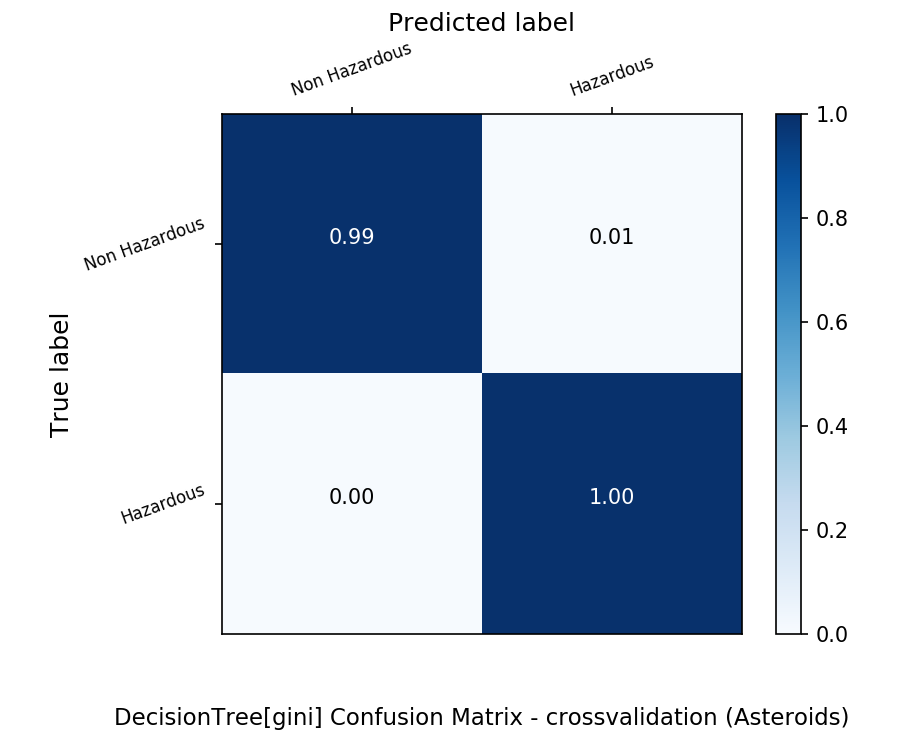
\includegraphics[width=1.1\textwidth]{Plots/asteroids/asteroids_DecisionTree_gini_balance_True_crossvalidation.png}
		\caption{balanced}
	\end{subfigure}%
	\begin{subfigure}{.5\textwidth}
		\centering
		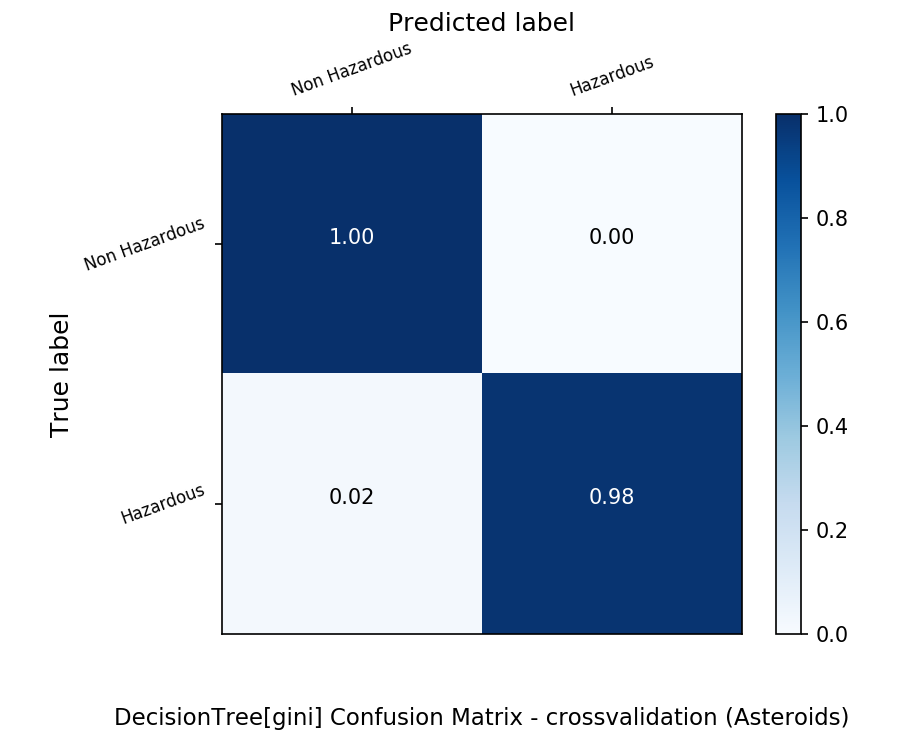
\includegraphics[width=1.1\textwidth]{Plots/asteroids/asteroids_DecisionTree_gini_balance_False_crossvalidation.png}
		\caption{non-balanced}
	\end{subfigure}
	\caption{{\color{red} PLACEHOLDER IMAGES. NEED TO BE CHANGED.}}
\end{figure}


\paragraph{Naive bayes}
We can notice that in our experimet there is no relevant difference in balancing the data if we apply a naive bayes classifier.
The main thing that we can notice is that the result obtained using cross validation is better than the oune obtained using holdout.


\begin{figure}[H]
	\centering
	\begin{subfigure}{.5\textwidth}
		\centering
		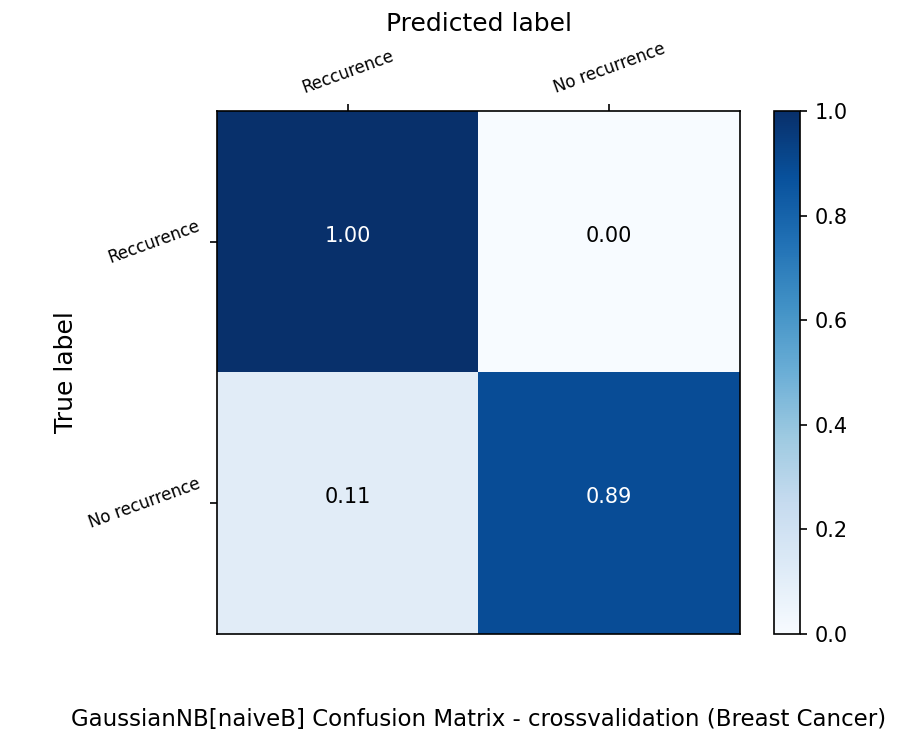
\includegraphics[width=1.1\textwidth]{Plots/breastCancer_GaussianNB_naiveB_balance_True_crossvalidation.png}
		\caption{balanced}
	\end{subfigure}%
	\begin{subfigure}{.5\textwidth}
		\centering
		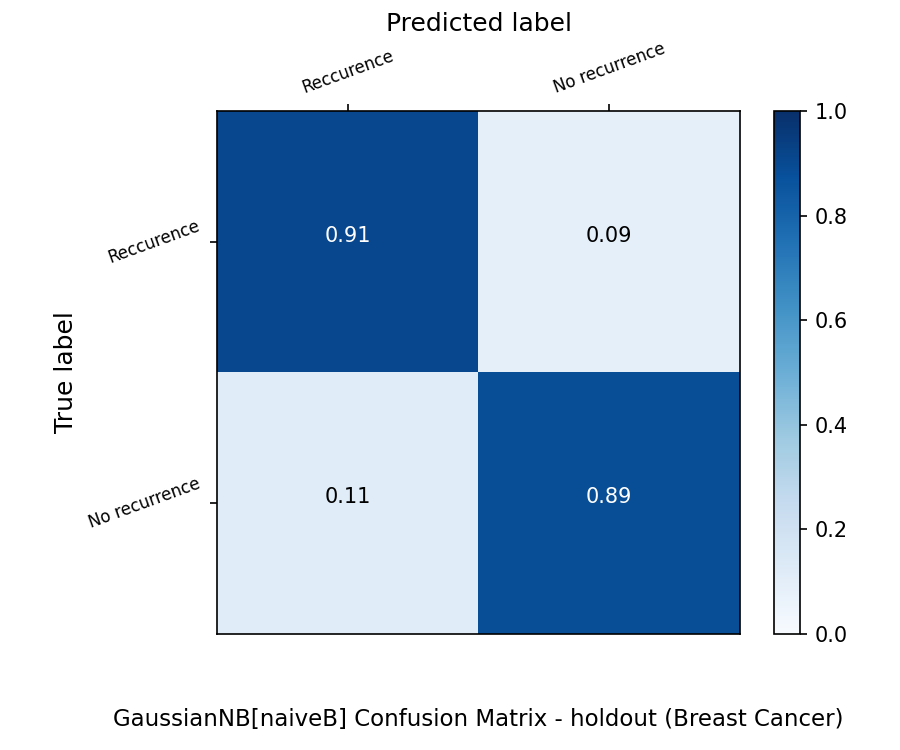
\includegraphics[width=1.1\textwidth]{Plots/breastCancer_GaussianNB_naiveB_balance_True_holdout.png}
		\caption{non-balanced}
	\end{subfigure}
	\caption{{\color{red} Comparison between Naive Bayes using cross validation and holdout.}}
\end{figure}


\paragraph{Decision trees}
When we compute the decision tree we can notice that the  accuracy value for a tree computed with the Gini index and the entropy  with cross validation are the same. Using the entropy we have a better outcome in the true positive while we do errors in the true negatives while we obtain the opposite while using the Gini index.


\begin{figure}[H]
	\centering
	\begin{subfigure}{.5\textwidth}
		\centering
		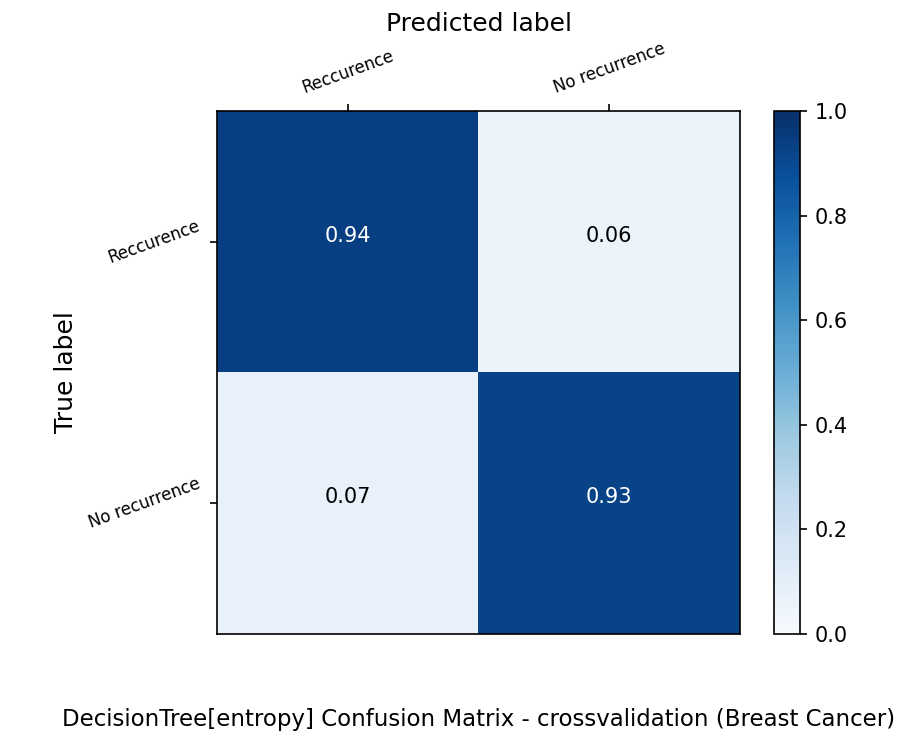
\includegraphics[width=1.1\textwidth]{Plots/breastCancer_DecisionTree_entropy_balance_True_crossvalidation.png}
		\caption{balanced}
	\end{subfigure}%
	\begin{subfigure}{.5\textwidth}
		\centering
		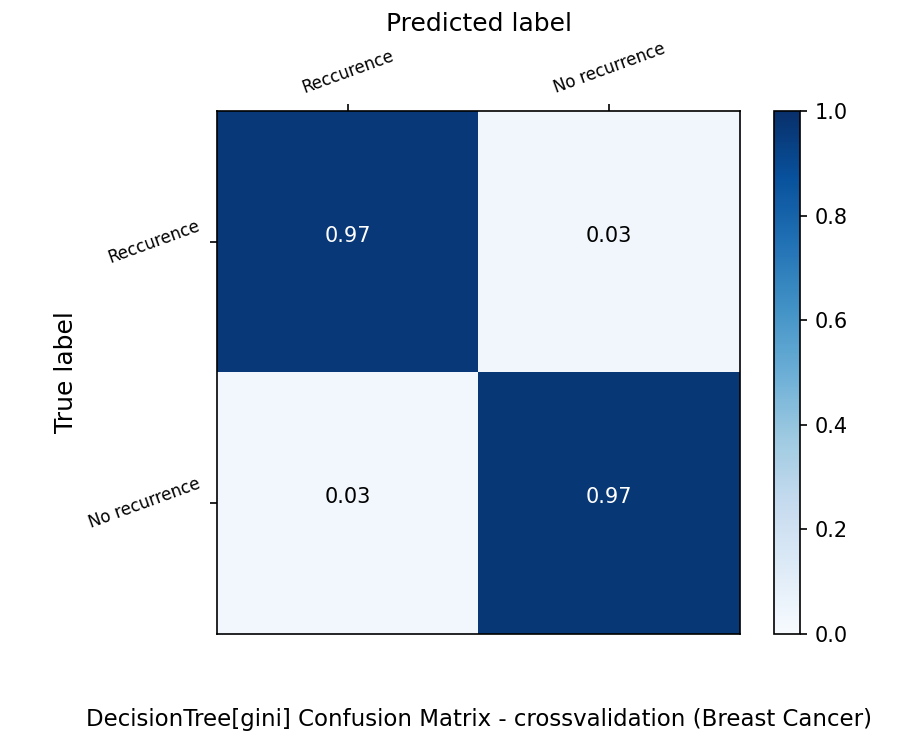
\includegraphics[width=1.1\textwidth]{Plots/breastCancer_DecisionTree_gini_balance_True_crossvalidation.png}
		\caption{non-balanced}
	\end{subfigure}
	\caption{{\color{red} Decision tree using entropy and Gini index .}}
\end{figure}


Using the holdout approach we can notice that we get better results using the entropy instead of the Gini index. If we train the classifier using balanced data from the experiment we can notice that we get better results. Looking at the results of the experiments we can notice that a good classifier is obtained using cross validation and the decision tree that uses the Gini index.





\clearpage
\bibliography{literature.bib}{}
\bibliographystyle{unsrt}

\newpage

\appendix
\section{Drug consumption - Confusion matrices}\label{app:drug_conf_matr}

\begin{figure}[H]
	\centering
	\begin{minipage}[b]{0.32\textwidth}
		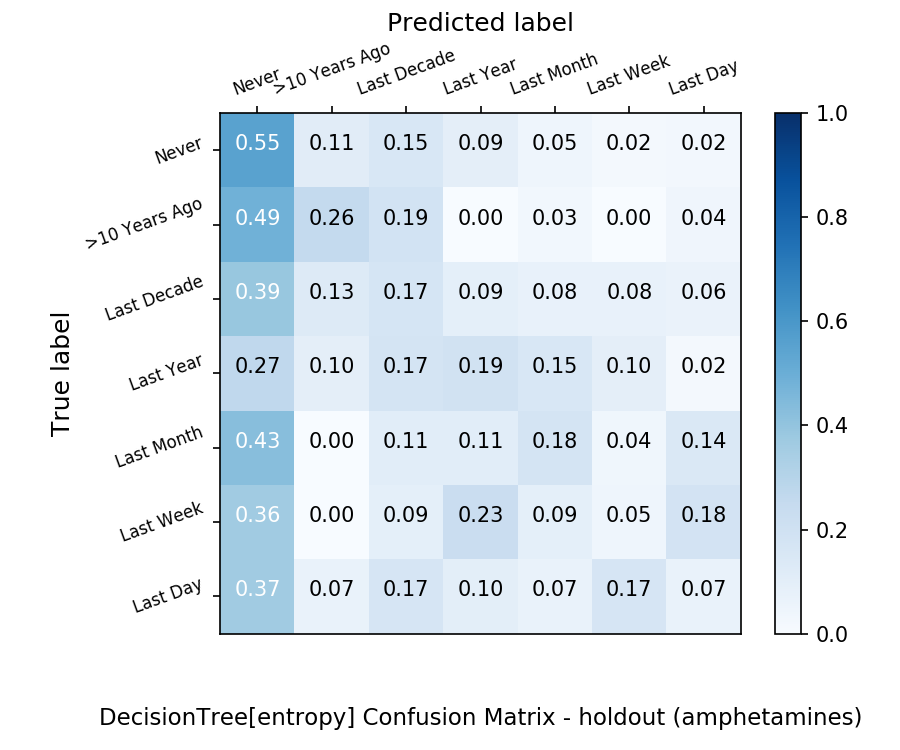
\includegraphics[width=1.1\textwidth]{Plots/amphetamines_DecisionTree_entropy_balance_False_holdout.png}
	\end{minipage}
	\begin{minipage}[b]{0.32\textwidth}
		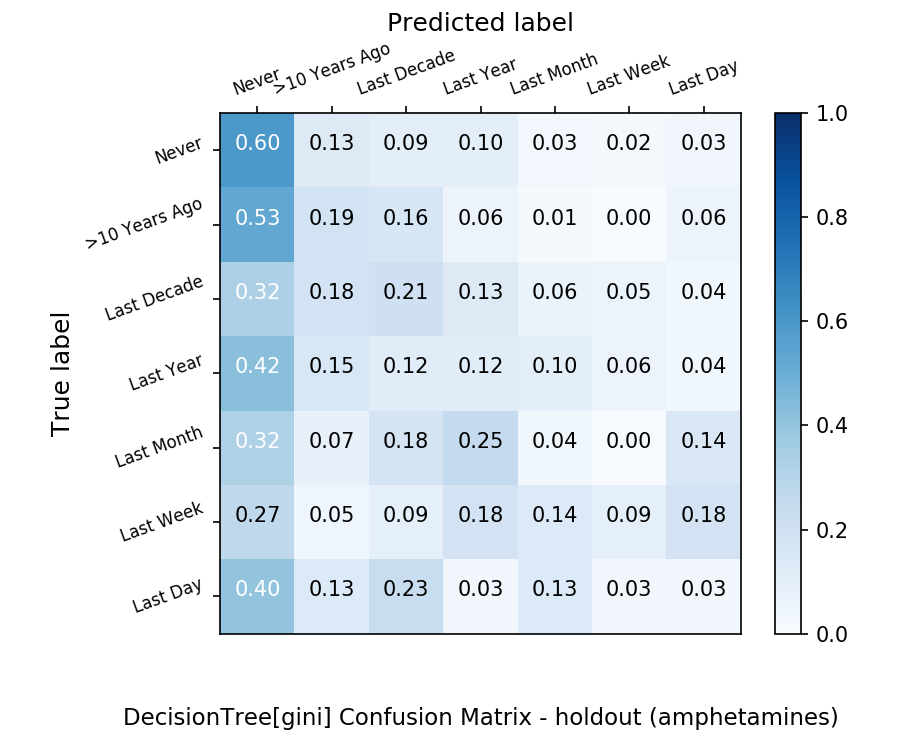
\includegraphics[width=1.1\textwidth]{Plots/amphetamines_DecisionTree_gini_balance_False_holdout.png}
	\end{minipage}
	\begin{minipage}[b]{0.32\textwidth}
		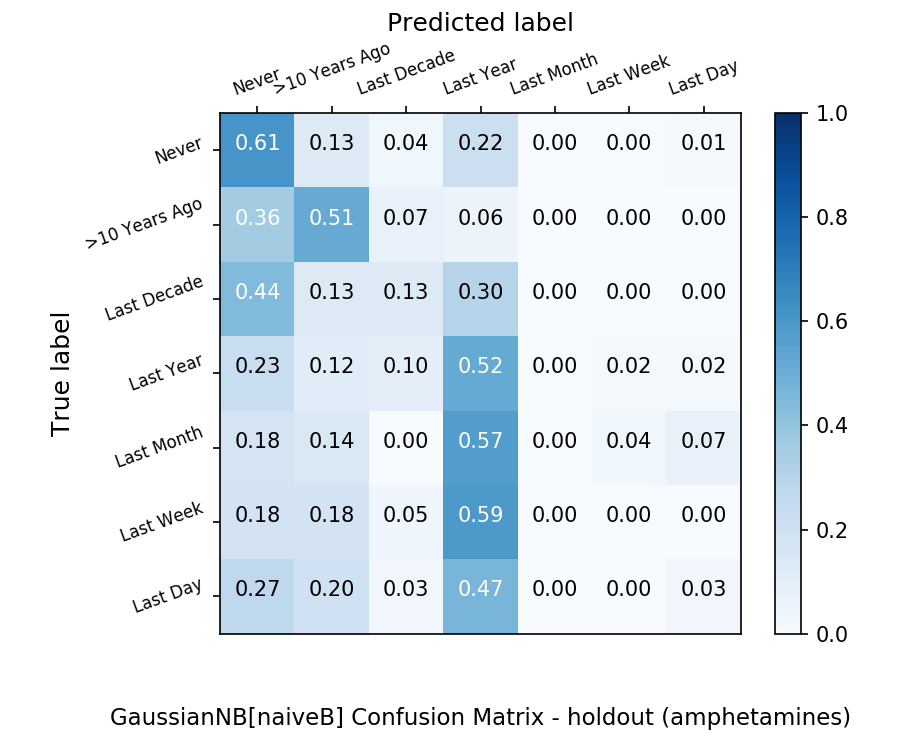
\includegraphics[width=1.1\textwidth]{Plots/amphetamines_GaussianNB_naiveB_balance_False_holdout.png}
	\end{minipage}
	\begin{minipage}[b]{0.32\textwidth}
		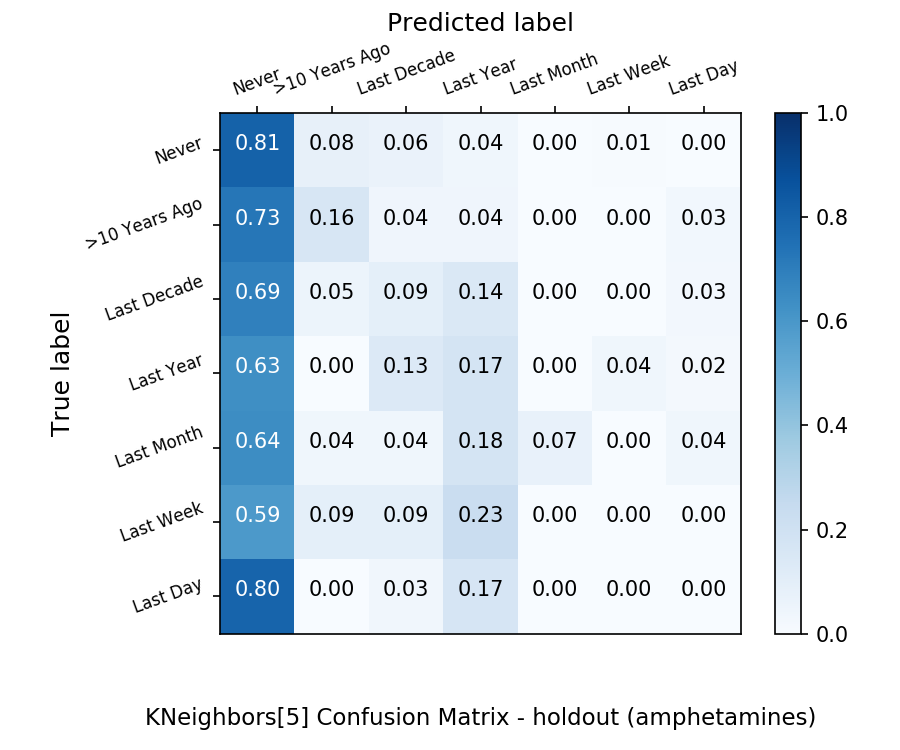
\includegraphics[width=1.1\textwidth]{Plots/amphetamines_KNeighbors_5_balance_False_holdout.png}
  \end{minipage}
	\begin{minipage}[b]{0.32\textwidth}
		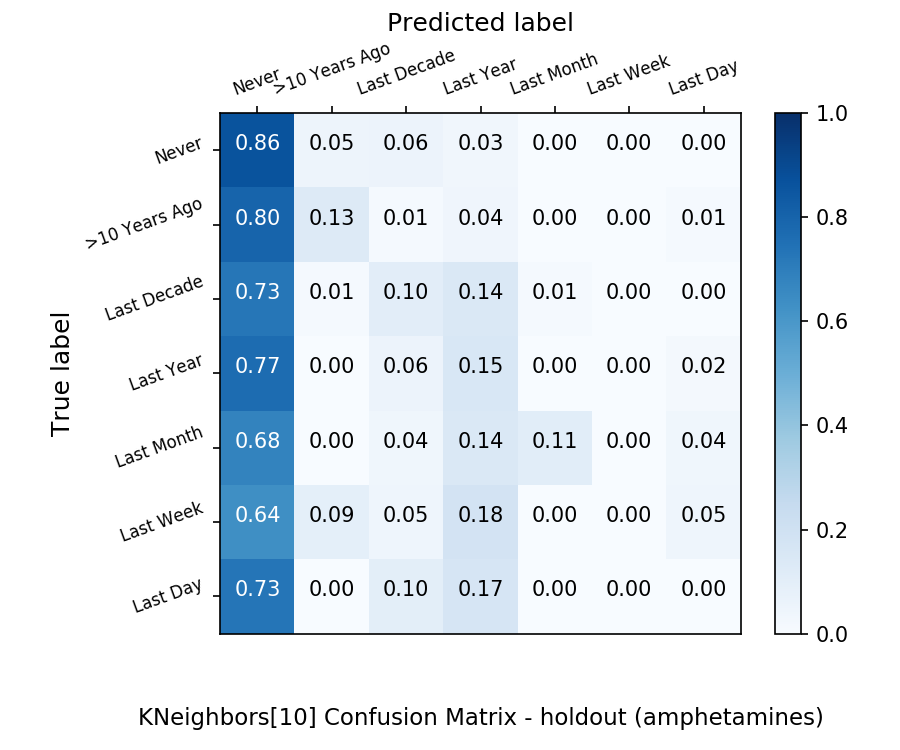
\includegraphics[width=1.1\textwidth]{Plots/amphetamines_KNeighbors_10_balance_False_holdout.png}
  \end{minipage}
	\begin{minipage}[b]{0.32\textwidth}
		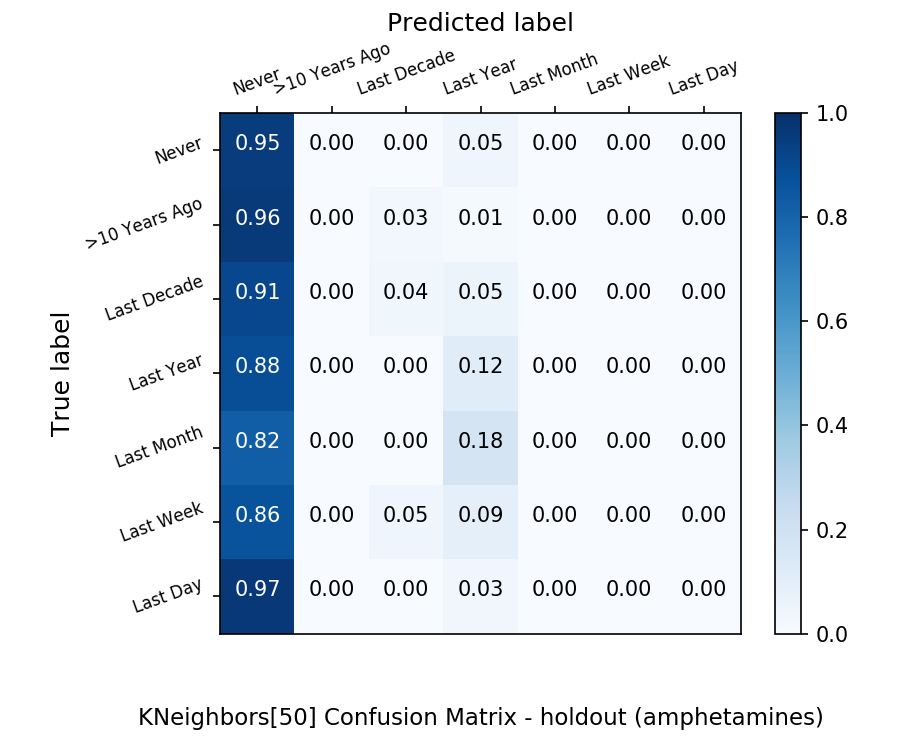
\includegraphics[width=1.1\textwidth]{Plots/amphetamines_KNeighbors_50_balance_False_holdout.png}
  \end{minipage}
	\caption{Confusion matrices for the used classifiers on the drug amphetamines.}
\end{figure}

\begin{figure}[H]
	\centering
	\begin{minipage}[b]{0.32\textwidth}
		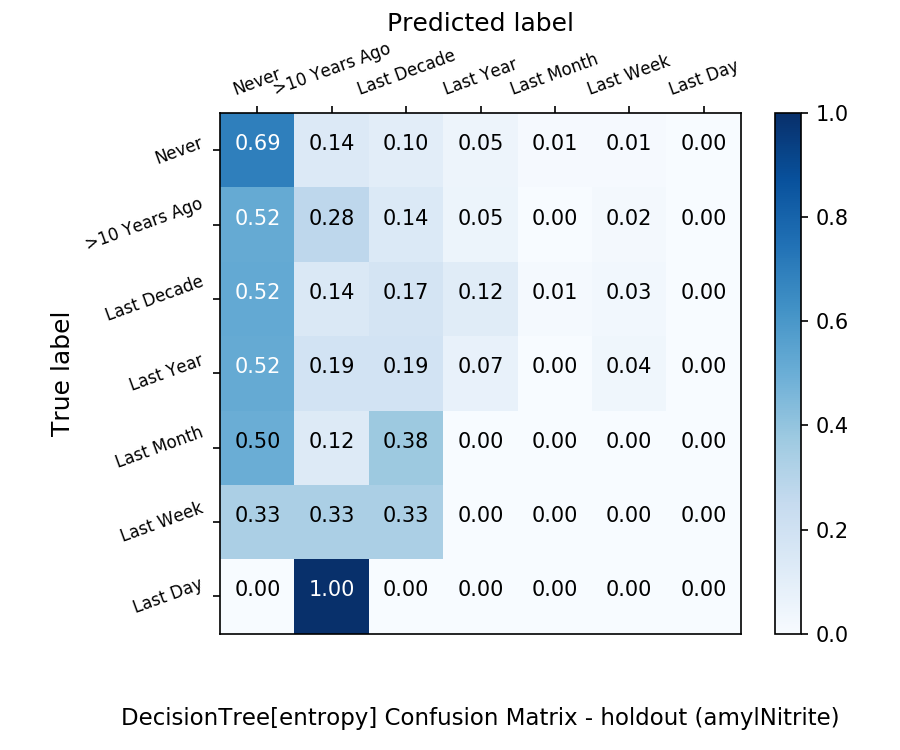
\includegraphics[width=1.1\textwidth]{Plots/amylNitrite_DecisionTree_entropy_balance_False_holdout.png}
	\end{minipage}
	\begin{minipage}[b]{0.32\textwidth}
		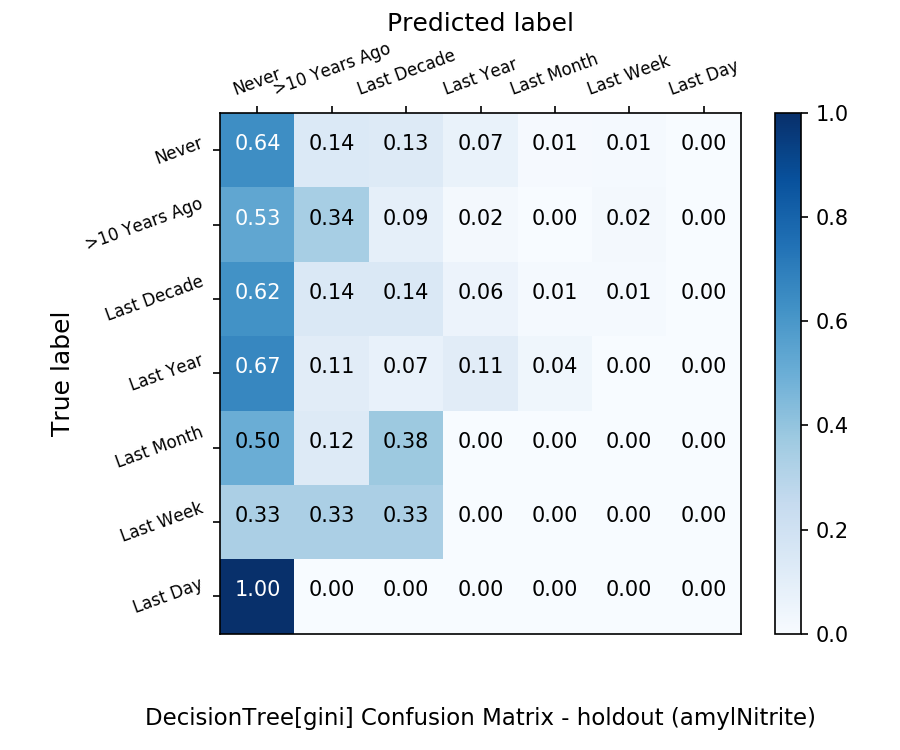
\includegraphics[width=1.1\textwidth]{Plots/amylNitrite_DecisionTree_gini_balance_False_holdout.png}
	\end{minipage}
	\begin{minipage}[b]{0.32\textwidth}
		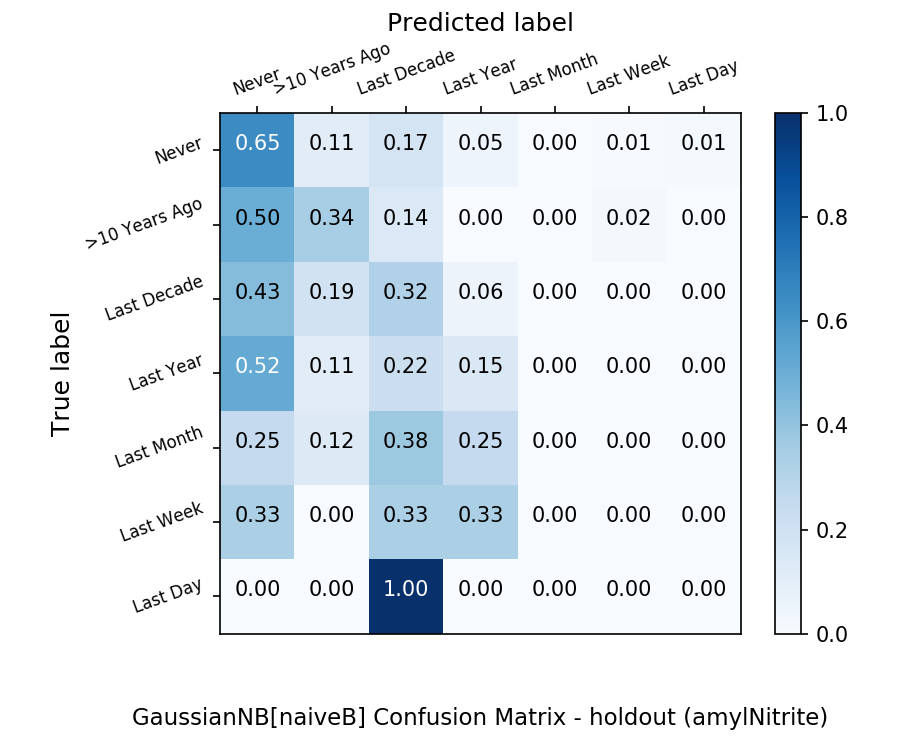
\includegraphics[width=1.1\textwidth]{Plots/amylNitrite_GaussianNB_naiveB_balance_False_holdout.png}
	\end{minipage}
	\begin{minipage}[b]{0.32\textwidth}
		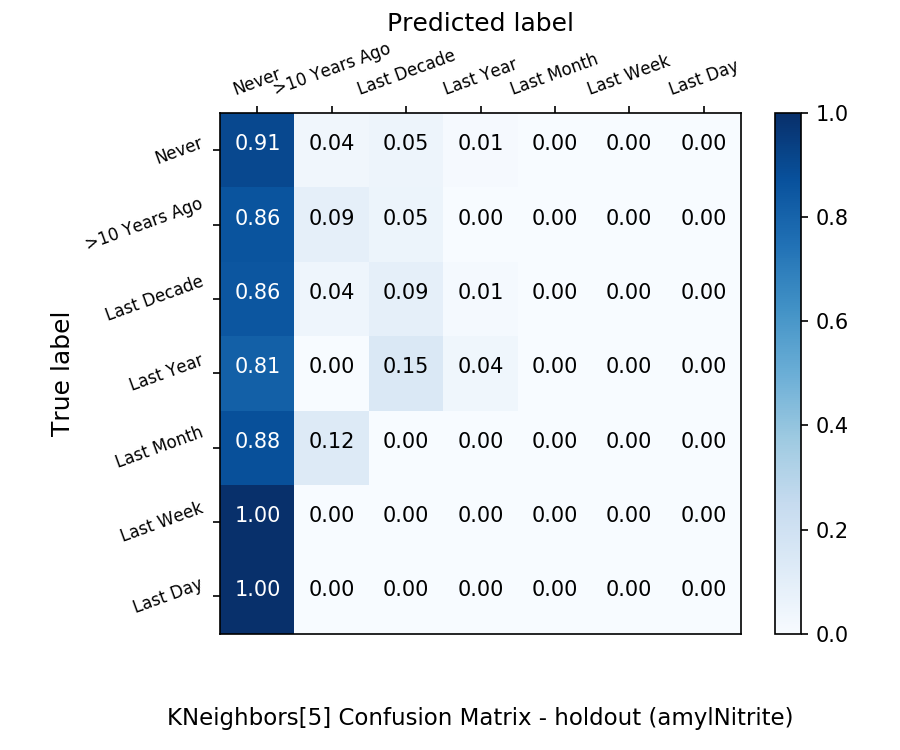
\includegraphics[width=1.1\textwidth]{Plots/amylNitrite_KNeighbors_5_balance_False_holdout.png}
  \end{minipage}
	\begin{minipage}[b]{0.32\textwidth}
		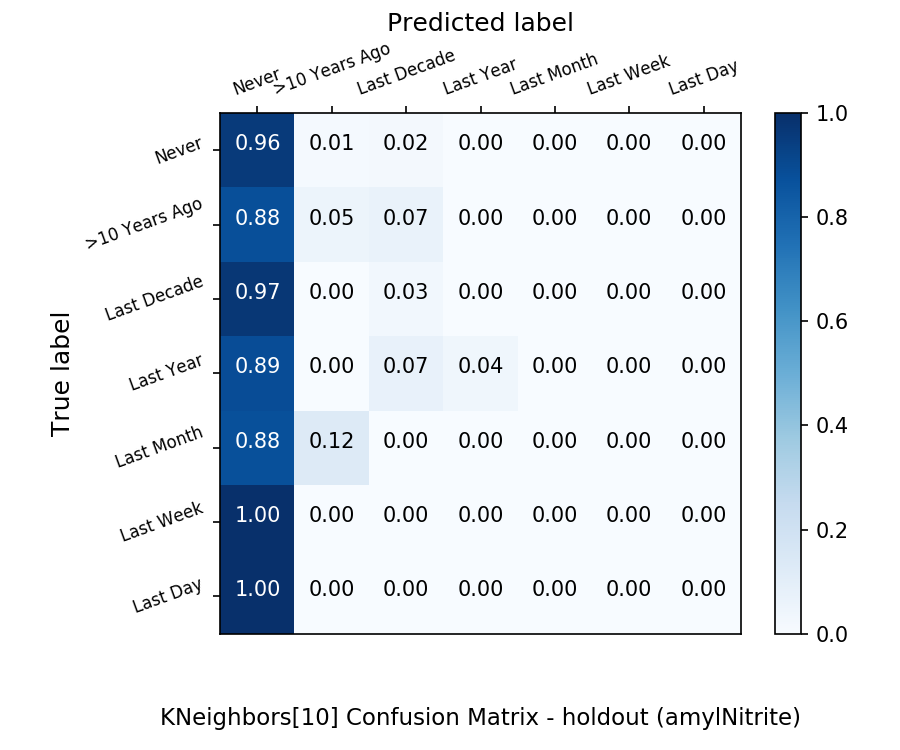
\includegraphics[width=1.1\textwidth]{Plots/amylNitrite_KNeighbors_10_balance_False_holdout.png}
  \end{minipage}
	\begin{minipage}[b]{0.32\textwidth}
		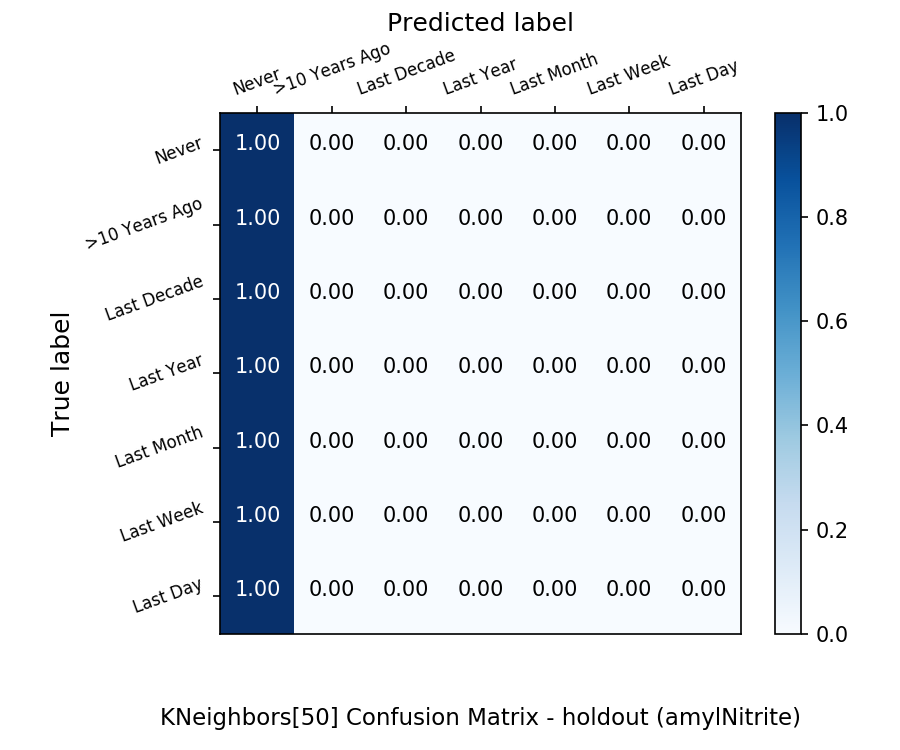
\includegraphics[width=1.1\textwidth]{Plots/amylNitrite_KNeighbors_50_balance_False_holdout.png}
  \end{minipage}
	\caption{Confusion matrices for the used classifiers on the drug amyl nitrite.}
\end{figure}

\begin{figure}[H]
	\centering
	\begin{minipage}[b]{0.32\textwidth}
		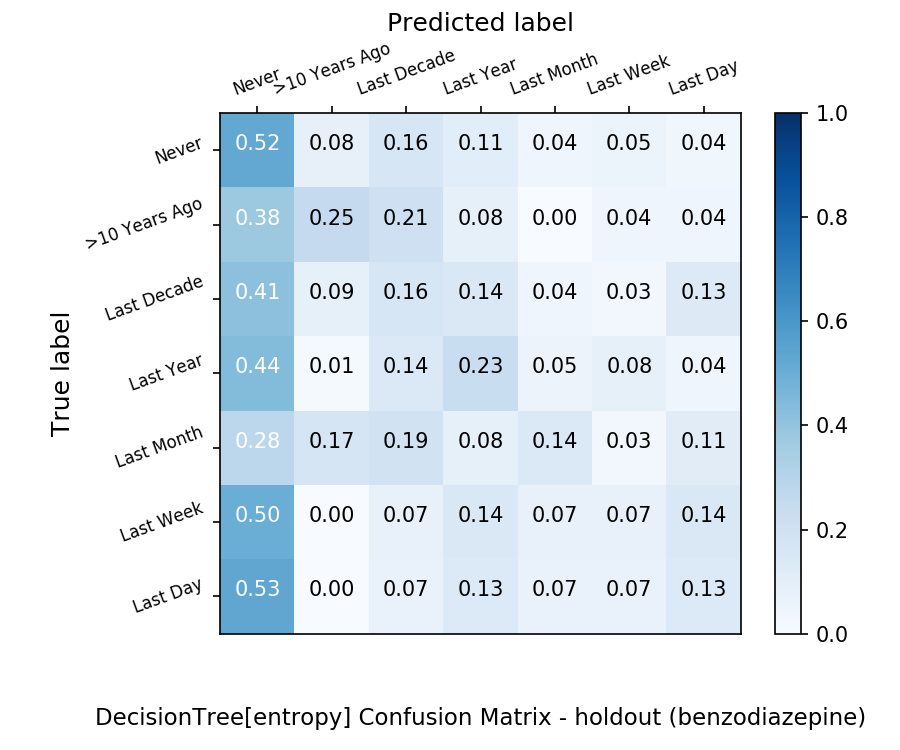
\includegraphics[width=1.1\textwidth]{Plots/benzodiazepine_DecisionTree_entropy_balance_False_holdout.png}
	\end{minipage}
	\begin{minipage}[b]{0.32\textwidth}
		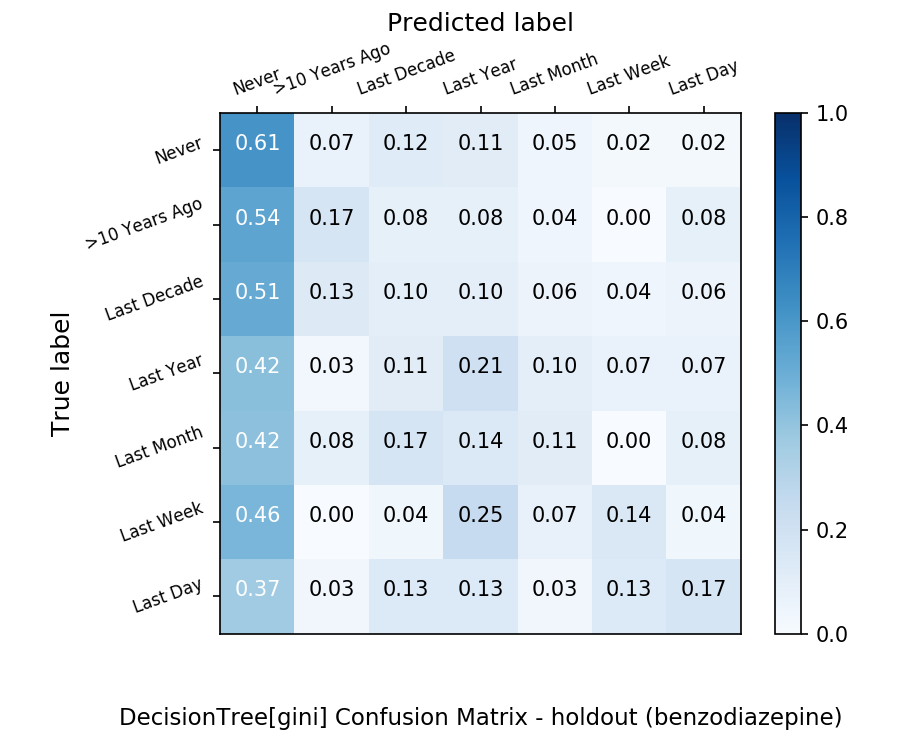
\includegraphics[width=1.1\textwidth]{Plots/benzodiazepine_DecisionTree_gini_balance_False_holdout.png}
	\end{minipage}
	\begin{minipage}[b]{0.32\textwidth}
		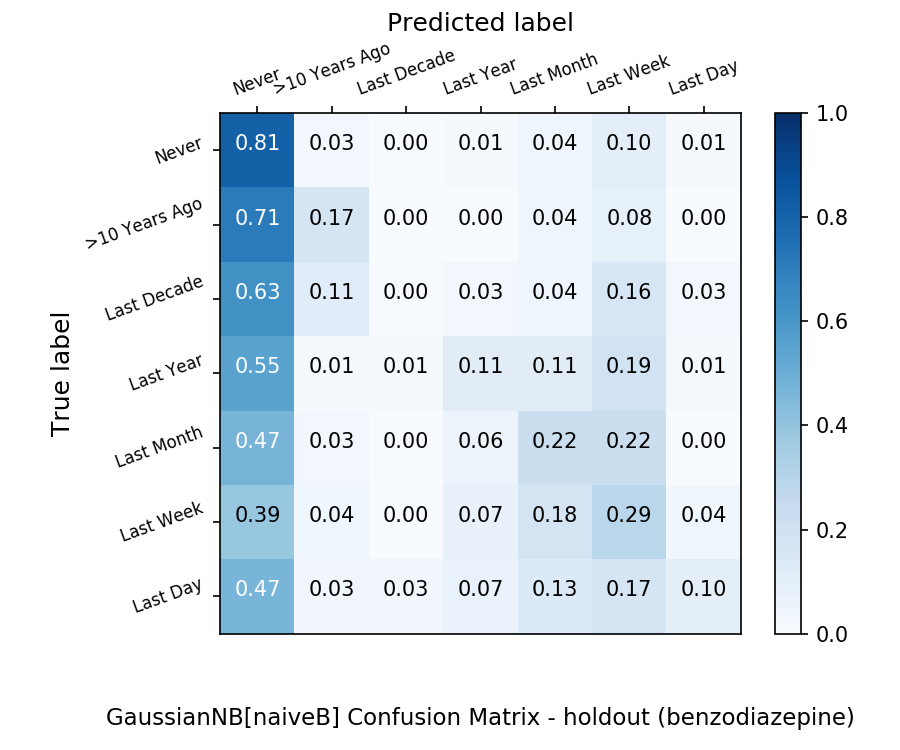
\includegraphics[width=1.1\textwidth]{Plots/benzodiazepine_GaussianNB_naiveB_balance_False_holdout.png}
	\end{minipage}
	\begin{minipage}[b]{0.32\textwidth}
		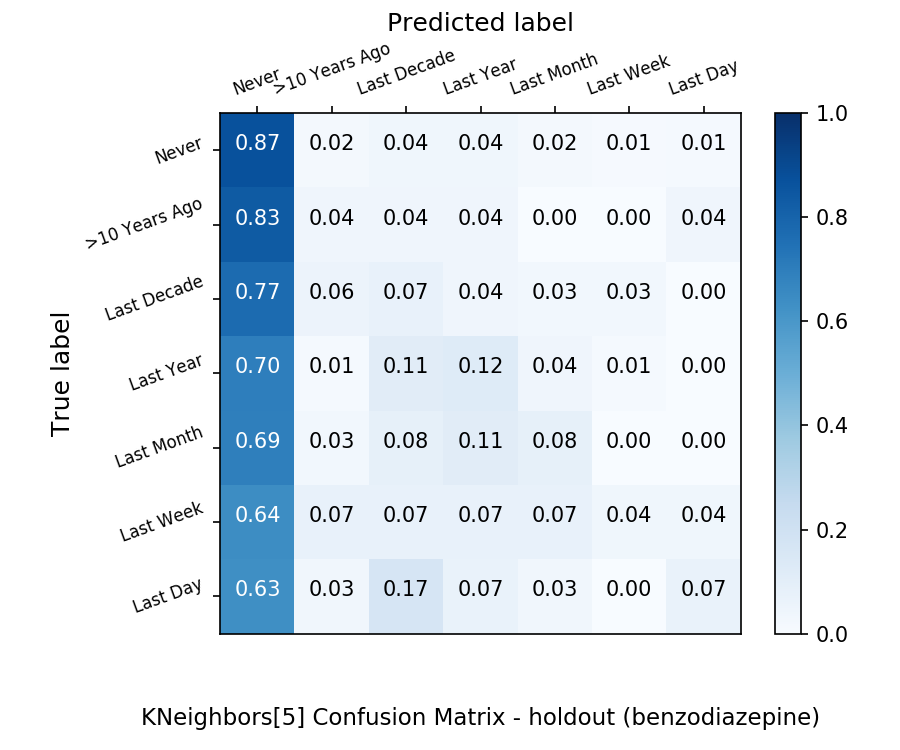
\includegraphics[width=1.1\textwidth]{Plots/benzodiazepine_KNeighbors_5_balance_False_holdout.png}
  \end{minipage}
	\begin{minipage}[b]{0.32\textwidth}
		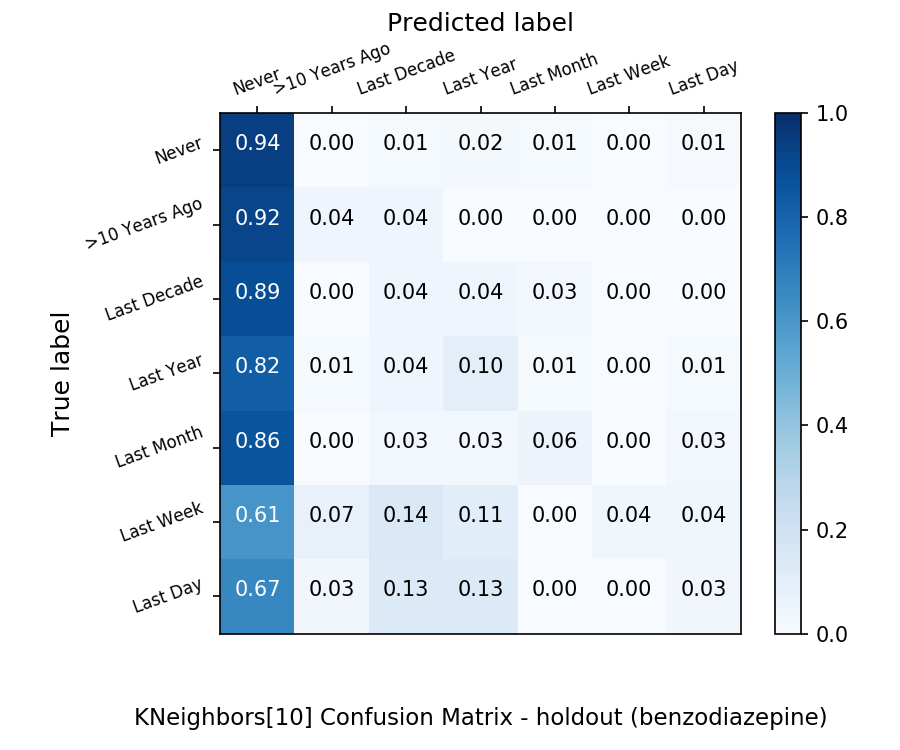
\includegraphics[width=1.1\textwidth]{Plots/benzodiazepine_KNeighbors_10_balance_False_holdout.png}
  \end{minipage}
	\begin{minipage}[b]{0.32\textwidth}
		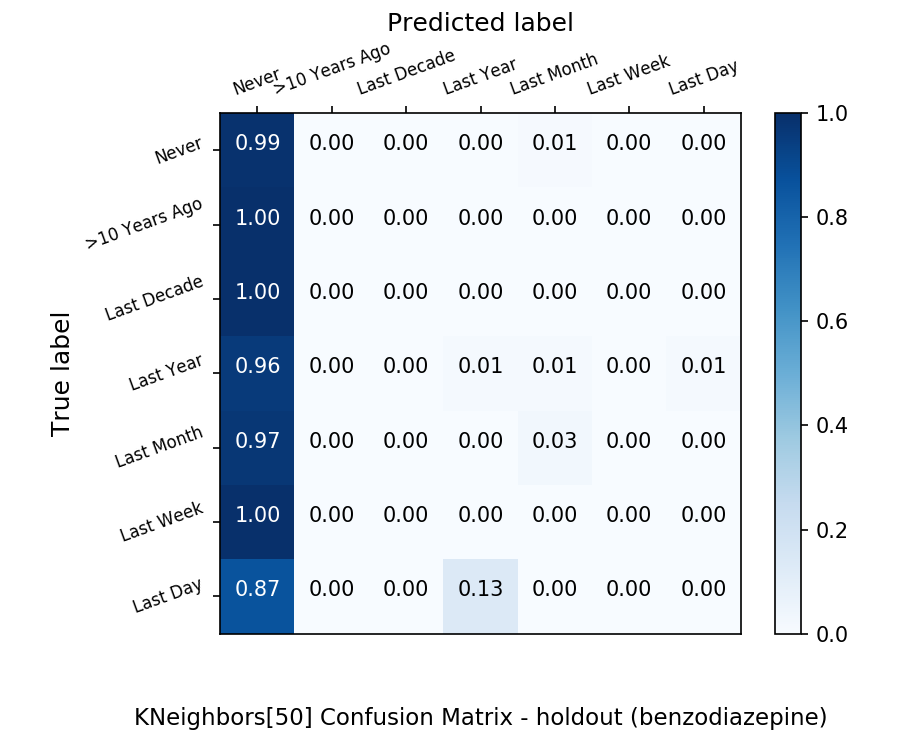
\includegraphics[width=1.1\textwidth]{Plots/benzodiazepine_KNeighbors_50_balance_False_holdout.png}
  \end{minipage}
	\caption{Confusion matrices for the used classifiers on the drug benzodiazepine.}
\end{figure}

\begin{figure}[H]
	\centering
	\begin{minipage}[b]{0.32\textwidth}
		\includegraphics[width=1.1\textwidth]{Plots/caffeine_DecisionTree_entropy_balance_False_holdout.png}
	\end{minipage}
	\begin{minipage}[b]{0.32\textwidth}
		\includegraphics[width=1.1\textwidth]{Plots/caffeine_DecisionTree_gini_balance_False_holdout.png}
	\end{minipage}
	\begin{minipage}[b]{0.32\textwidth}
		\includegraphics[width=1.1\textwidth]{Plots/caffeine_GaussianNB_naiveB_balance_False_holdout.png}
	\end{minipage}
	\begin{minipage}[b]{0.32\textwidth}
		\includegraphics[width=1.1\textwidth]{Plots/caffeine_KNeighbors_5_balance_False_holdout.png}
  \end{minipage}
	\begin{minipage}[b]{0.32\textwidth}
		\includegraphics[width=1.1\textwidth]{Plots/caffeine_KNeighbors_10_balance_False_holdout.png}
  \end{minipage}
	\begin{minipage}[b]{0.32\textwidth}
		\includegraphics[width=1.1\textwidth]{Plots/caffeine_KNeighbors_50_balance_False_holdout.png}
  \end{minipage}
	\caption{Confusion matrices for the used classifiers on the drug caffeine.}
\end{figure}

\begin{figure}[H]
	\centering
	\begin{minipage}[b]{0.32\textwidth}
		\includegraphics[width=1.1\textwidth]{Plots/cannabis_DecisionTree_entropy_balance_False_holdout.png}
	\end{minipage}
	\begin{minipage}[b]{0.32\textwidth}
		\includegraphics[width=1.1\textwidth]{Plots/cannabis_DecisionTree_gini_balance_False_holdout.png}
	\end{minipage}
	\begin{minipage}[b]{0.32\textwidth}
		\includegraphics[width=1.1\textwidth]{Plots/cannabis_GaussianNB_naiveB_balance_False_holdout.png}
	\end{minipage}
	\begin{minipage}[b]{0.32\textwidth}
		\includegraphics[width=1.1\textwidth]{Plots/cannabis_KNeighbors_5_balance_False_holdout.png}
  \end{minipage}
	\begin{minipage}[b]{0.32\textwidth}
		\includegraphics[width=1.1\textwidth]{Plots/cannabis_KNeighbors_10_balance_False_holdout.png}
  \end{minipage}
	\begin{minipage}[b]{0.32\textwidth}
		\includegraphics[width=1.1\textwidth]{Plots/cannabis_KNeighbors_50_balance_False_holdout.png}
  \end{minipage}
	\caption{Confusion matrices for the used classifiers on the drug cannabis.}
\end{figure}

\begin{figure}[H]
	\centering
	\begin{minipage}[b]{0.32\textwidth}
		\includegraphics[width=1.1\textwidth]{Plots/chocolate_DecisionTree_entropy_balance_False_holdout.png}
	\end{minipage}
	\begin{minipage}[b]{0.32\textwidth}
		\includegraphics[width=1.1\textwidth]{Plots/chocolate_DecisionTree_gini_balance_False_holdout.png}
	\end{minipage}
	\begin{minipage}[b]{0.32\textwidth}
		\includegraphics[width=1.1\textwidth]{Plots/chocolate_GaussianNB_naiveB_balance_False_holdout.png}
	\end{minipage}
	\begin{minipage}[b]{0.32\textwidth}
		\includegraphics[width=1.1\textwidth]{Plots/chocolate_KNeighbors_5_balance_False_holdout.png}
  \end{minipage}
	\begin{minipage}[b]{0.32\textwidth}
		\includegraphics[width=1.1\textwidth]{Plots/chocolate_KNeighbors_10_balance_False_holdout.png}
  \end{minipage}
	\begin{minipage}[b]{0.32\textwidth}
		\includegraphics[width=1.1\textwidth]{Plots/chocolate_KNeighbors_50_balance_False_holdout.png}
  \end{minipage}
	\caption{Confusion matrices for the used classifiers on the drug chocolate.}
\end{figure}

\begin{figure}[H]
	\centering
	\begin{minipage}[b]{0.32\textwidth}
		\includegraphics[width=1.1\textwidth]{Plots/cocaine_DecisionTree_entropy_balance_False_holdout.png}
	\end{minipage}
	\begin{minipage}[b]{0.32\textwidth}
		\includegraphics[width=1.1\textwidth]{Plots/cocaine_DecisionTree_gini_balance_False_holdout.png}
	\end{minipage}
	\begin{minipage}[b]{0.32\textwidth}
		\includegraphics[width=1.1\textwidth]{Plots/cocaine_GaussianNB_naiveB_balance_False_holdout.png}
	\end{minipage}
	\begin{minipage}[b]{0.32\textwidth}
		\includegraphics[width=1.1\textwidth]{Plots/cocaine_KNeighbors_5_balance_False_holdout.png}
  \end{minipage}
	\begin{minipage}[b]{0.32\textwidth}
		\includegraphics[width=1.1\textwidth]{Plots/cocaine_KNeighbors_10_balance_False_holdout.png}
  \end{minipage}
	\begin{minipage}[b]{0.32\textwidth}
		\includegraphics[width=1.1\textwidth]{Plots/cocaine_KNeighbors_50_balance_False_holdout.png}
  \end{minipage}
	\caption{Confusion matrices for the used classifiers on the drug cocaine.}
\end{figure}

\begin{figure}[H]
	\centering
	\begin{minipage}[b]{0.32\textwidth}
		\includegraphics[width=1.1\textwidth]{Plots/crack_DecisionTree_entropy_balance_False_holdout.png}
	\end{minipage}
	\begin{minipage}[b]{0.32\textwidth}
		\includegraphics[width=1.1\textwidth]{Plots/crack_DecisionTree_gini_balance_False_holdout.png}
	\end{minipage}
	\begin{minipage}[b]{0.32\textwidth}
		\includegraphics[width=1.1\textwidth]{Plots/crack_GaussianNB_naiveB_balance_False_holdout.png}
	\end{minipage}
	\begin{minipage}[b]{0.32\textwidth}
		\includegraphics[width=1.1\textwidth]{Plots/crack_KNeighbors_5_balance_False_holdout.png}
  \end{minipage}
	\begin{minipage}[b]{0.32\textwidth}
		\includegraphics[width=1.1\textwidth]{Plots/crack_KNeighbors_10_balance_False_holdout.png}
  \end{minipage}
	\begin{minipage}[b]{0.32\textwidth}
		\includegraphics[width=1.1\textwidth]{Plots/crack_KNeighbors_50_balance_False_holdout.png}
  \end{minipage}
	\caption{Confusion matrices for the used classifiers on the drug crack.}
\end{figure}

\begin{figure}[H]
	\centering
	\begin{minipage}[b]{0.32\textwidth}
		\includegraphics[width=1.1\textwidth]{Plots/ecstasy_DecisionTree_entropy_balance_False_holdout.png}
	\end{minipage}
	\begin{minipage}[b]{0.32\textwidth}
		\includegraphics[width=1.1\textwidth]{Plots/ecstasy_DecisionTree_gini_balance_False_holdout.png}
	\end{minipage}
	\begin{minipage}[b]{0.32\textwidth}
		\includegraphics[width=1.1\textwidth]{Plots/ecstasy_GaussianNB_naiveB_balance_False_holdout.png}
	\end{minipage}
	\begin{minipage}[b]{0.32\textwidth}
		\includegraphics[width=1.1\textwidth]{Plots/ecstasy_KNeighbors_5_balance_False_holdout.png}
  \end{minipage}
	\begin{minipage}[b]{0.32\textwidth}
		\includegraphics[width=1.1\textwidth]{Plots/ecstasy_KNeighbors_10_balance_False_holdout.png}
  \end{minipage}
	\begin{minipage}[b]{0.32\textwidth}
		\includegraphics[width=1.1\textwidth]{Plots/ecstasy_KNeighbors_50_balance_False_holdout.png}
  \end{minipage}
	\caption{Confusion matrices for the used classifiers on the drug ecstasy.}
\end{figure}

\begin{figure}[H]
	\centering
	\begin{minipage}[b]{0.32\textwidth}
		\includegraphics[width=1.1\textwidth]{Plots/heroin_DecisionTree_entropy_balance_False_holdout.png}
	\end{minipage}
	\begin{minipage}[b]{0.32\textwidth}
		\includegraphics[width=1.1\textwidth]{Plots/heroin_DecisionTree_gini_balance_False_holdout.png}
	\end{minipage}
	\begin{minipage}[b]{0.32\textwidth}
		\includegraphics[width=1.1\textwidth]{Plots/heroin_GaussianNB_naiveB_balance_False_holdout.png}
	\end{minipage}
	\begin{minipage}[b]{0.32\textwidth}
		\includegraphics[width=1.1\textwidth]{Plots/heroin_KNeighbors_5_balance_False_holdout.png}
  \end{minipage}
	\begin{minipage}[b]{0.32\textwidth}
		\includegraphics[width=1.1\textwidth]{Plots/heroin_KNeighbors_10_balance_False_holdout.png}
  \end{minipage}
	\begin{minipage}[b]{0.32\textwidth}
		\includegraphics[width=1.1\textwidth]{Plots/heroin_KNeighbors_50_balance_False_holdout.png}
  \end{minipage}
	\caption{Confusion matrices for the used classifiers on the drug heroin.}
\end{figure}

\begin{figure}[H]
	\centering
	\begin{minipage}[b]{0.32\textwidth}
		\includegraphics[width=1.1\textwidth]{Plots/ketamine_DecisionTree_entropy_balance_False_holdout.png}
	\end{minipage}
	\begin{minipage}[b]{0.32\textwidth}
		\includegraphics[width=1.1\textwidth]{Plots/ketamine_DecisionTree_gini_balance_False_holdout.png}
	\end{minipage}
	\begin{minipage}[b]{0.32\textwidth}
		\includegraphics[width=1.1\textwidth]{Plots/ketamine_GaussianNB_naiveB_balance_False_holdout.png}
	\end{minipage}
	\begin{minipage}[b]{0.32\textwidth}
		\includegraphics[width=1.1\textwidth]{Plots/ketamine_KNeighbors_5_balance_False_holdout.png}
  \end{minipage}
	\begin{minipage}[b]{0.32\textwidth}
		\includegraphics[width=1.1\textwidth]{Plots/ketamine_KNeighbors_10_balance_False_holdout.png}
  \end{minipage}
	\begin{minipage}[b]{0.32\textwidth}
		\includegraphics[width=1.1\textwidth]{Plots/ketamine_KNeighbors_50_balance_False_holdout.png}
  \end{minipage}
	\caption{Confusion matrices for the used classifiers on the drug ketamine.}
\end{figure}

\begin{figure}[H]
	\centering
	\begin{minipage}[b]{0.32\textwidth}
		\includegraphics[width=1.1\textwidth]{Plots/legal_DecisionTree_entropy_balance_False_holdout.png}
	\end{minipage}
	\begin{minipage}[b]{0.32\textwidth}
		\includegraphics[width=1.1\textwidth]{Plots/legal_DecisionTree_gini_balance_False_holdout.png}
	\end{minipage}
	\begin{minipage}[b]{0.32\textwidth}
		\includegraphics[width=1.1\textwidth]{Plots/legal_GaussianNB_naiveB_balance_False_holdout.png}
	\end{minipage}
	\begin{minipage}[b]{0.32\textwidth}
		\includegraphics[width=1.1\textwidth]{Plots/legal_KNeighbors_5_balance_False_holdout.png}
  \end{minipage}
	\begin{minipage}[b]{0.32\textwidth}
		\includegraphics[width=1.1\textwidth]{Plots/legal_KNeighbors_10_balance_False_holdout.png}
  \end{minipage}
	\begin{minipage}[b]{0.32\textwidth}
		\includegraphics[width=1.1\textwidth]{Plots/legal_KNeighbors_50_balance_False_holdout.png}
  \end{minipage}
	\caption{Confusion matrices for the used classifiers on the drug legal.}
\end{figure}

\begin{figure}[H]
	\centering
	\begin{minipage}[b]{0.32\textwidth}
		\includegraphics[width=1.1\textwidth]{Plots/LSD_DecisionTree_entropy_balance_False_holdout.png}
	\end{minipage}
	\begin{minipage}[b]{0.32\textwidth}
		\includegraphics[width=1.1\textwidth]{Plots/LSD_DecisionTree_gini_balance_False_holdout.png}
	\end{minipage}
	\begin{minipage}[b]{0.32\textwidth}
		\includegraphics[width=1.1\textwidth]{Plots/LSD_GaussianNB_naiveB_balance_False_holdout.png}
	\end{minipage}
	\begin{minipage}[b]{0.32\textwidth}
		\includegraphics[width=1.1\textwidth]{Plots/LSD_KNeighbors_5_balance_False_holdout.png}
  \end{minipage}
	\begin{minipage}[b]{0.32\textwidth}
		\includegraphics[width=1.1\textwidth]{Plots/LSD_KNeighbors_10_balance_False_holdout.png}
  \end{minipage}
	\begin{minipage}[b]{0.32\textwidth}
		\includegraphics[width=1.1\textwidth]{Plots/LSD_KNeighbors_50_balance_False_holdout.png}
  \end{minipage}
	\caption{Confusion matrices for the used classifiers on the drug LSD.}
\end{figure}

\begin{figure}[H]
	\centering
	\begin{minipage}[b]{0.32\textwidth}
		\includegraphics[width=1.1\textwidth]{Plots/methadone_DecisionTree_entropy_balance_False_holdout.png}
	\end{minipage}
	\begin{minipage}[b]{0.32\textwidth}
		\includegraphics[width=1.1\textwidth]{Plots/methadone_DecisionTree_gini_balance_False_holdout.png}
	\end{minipage}
	\begin{minipage}[b]{0.32\textwidth}
		\includegraphics[width=1.1\textwidth]{Plots/methadone_GaussianNB_naiveB_balance_False_holdout.png}
	\end{minipage}
	\begin{minipage}[b]{0.32\textwidth}
		\includegraphics[width=1.1\textwidth]{Plots/methadone_KNeighbors_5_balance_False_holdout.png}
  \end{minipage}
	\begin{minipage}[b]{0.32\textwidth}
		\includegraphics[width=1.1\textwidth]{Plots/methadone_KNeighbors_10_balance_False_holdout.png}
  \end{minipage}
	\begin{minipage}[b]{0.32\textwidth}
		\includegraphics[width=1.1\textwidth]{Plots/methadone_KNeighbors_50_balance_False_holdout.png}
  \end{minipage}
	\caption{Confusion matrices for the used classifiers on the drug methadone.}
\end{figure}

\begin{figure}[H]
	\centering
	\begin{minipage}[b]{0.32\textwidth}
		\includegraphics[width=1.1\textwidth]{Plots/mushrooms_DecisionTree_entropy_balance_False_holdout.png}
	\end{minipage}
	\begin{minipage}[b]{0.32\textwidth}
		\includegraphics[width=1.1\textwidth]{Plots/mushrooms_DecisionTree_gini_balance_False_holdout.png}
	\end{minipage}
	\begin{minipage}[b]{0.32\textwidth}
		\includegraphics[width=1.1\textwidth]{Plots/mushrooms_GaussianNB_naiveB_balance_False_holdout.png}
	\end{minipage}
	\begin{minipage}[b]{0.32\textwidth}
		\includegraphics[width=1.1\textwidth]{Plots/mushrooms_KNeighbors_5_balance_False_holdout.png}
  \end{minipage}
	\begin{minipage}[b]{0.32\textwidth}
		\includegraphics[width=1.1\textwidth]{Plots/mushrooms_KNeighbors_10_balance_False_holdout.png}
  \end{minipage}
	\begin{minipage}[b]{0.32\textwidth}
		\includegraphics[width=1.1\textwidth]{Plots/mushrooms_KNeighbors_50_balance_False_holdout.png}
  \end{minipage}
	\caption{Confusion matrices for the used classifiers on the drug mushrooms.}
\end{figure}

\begin{figure}[H]
	\centering
	\begin{minipage}[b]{0.32\textwidth}
		\includegraphics[width=1.1\textwidth]{Plots/nicotine_DecisionTree_entropy_balance_False_holdout.png}
	\end{minipage}
	\begin{minipage}[b]{0.32\textwidth}
		\includegraphics[width=1.1\textwidth]{Plots/nicotine_DecisionTree_gini_balance_False_holdout.png}
	\end{minipage}
	\begin{minipage}[b]{0.32\textwidth}
		\includegraphics[width=1.1\textwidth]{Plots/nicotine_GaussianNB_naiveB_balance_False_holdout.png}
	\end{minipage}
	\begin{minipage}[b]{0.32\textwidth}
		\includegraphics[width=1.1\textwidth]{Plots/nicotine_KNeighbors_5_balance_False_holdout.png}
  \end{minipage}
	\begin{minipage}[b]{0.32\textwidth}
		\includegraphics[width=1.1\textwidth]{Plots/nicotine_KNeighbors_10_balance_False_holdout.png}
  \end{minipage}
	\begin{minipage}[b]{0.32\textwidth}
		\includegraphics[width=1.1\textwidth]{Plots/nicotine_KNeighbors_50_balance_False_holdout.png}
  \end{minipage}
	\caption{Confusion matrices for the used classifiers on the drug nicotine.}
\end{figure}

\begin{figure}[H]
	\centering
	\begin{minipage}[b]{0.32\textwidth}
		\includegraphics[width=1.1\textwidth]{Plots/volatileSubstance_DecisionTree_entropy_balance_False_holdout.png}
	\end{minipage}
	\begin{minipage}[b]{0.32\textwidth}
		\includegraphics[width=1.1\textwidth]{Plots/volatileSubstance_DecisionTree_gini_balance_False_holdout.png}
	\end{minipage}
	\begin{minipage}[b]{0.32\textwidth}
		\includegraphics[width=1.1\textwidth]{Plots/volatileSubstance_GaussianNB_naiveB_balance_False_holdout.png}
	\end{minipage}
	\begin{minipage}[b]{0.32\textwidth}
		\includegraphics[width=1.1\textwidth]{Plots/volatileSubstance_KNeighbors_5_balance_False_holdout.png}
  \end{minipage}
	\begin{minipage}[b]{0.32\textwidth}
		\includegraphics[width=1.1\textwidth]{Plots/volatileSubstance_KNeighbors_10_balance_False_holdout.png}
  \end{minipage}
	\begin{minipage}[b]{0.32\textwidth}
		\includegraphics[width=1.1\textwidth]{Plots/volatileSubstance_KNeighbors_50_balance_False_holdout.png}
  \end{minipage}
	\caption{Confusion matrices for the used classifiers on the drug volatile substance.}
\end{figure}

\section{Asteroids classification - Confusion matrices}\label{app:asteroids_conf_matr}

\begin{figure}[H]
	\centering
	\begin{subfigure}{.5\textwidth}
		\centering
		\includegraphics[width=1.1\textwidth]{Plots/asteroids/asteroids_GaussianNB_naiveB_balance_True_holdout.png}
		\caption{balanced}
	\end{subfigure}%
	\begin{subfigure}{.5\textwidth}
		\centering
		\includegraphics[width=1.1\textwidth]{Plots/asteroids/asteroids_GaussianNB_naiveB_balance_False_holdout.png}
		\caption{non-balanced}
	\end{subfigure}
\end{figure}

\begin{figure}[H]
	\centering
	\begin{subfigure}{.5\textwidth}
		\centering
		\includegraphics[width=1.1\textwidth]{Plots/asteroids/asteroids_GaussianNB_naiveB_balance_True_crossvalidation.png}
		\caption{balanced}
	\end{subfigure}%
	\begin{subfigure}{.5\textwidth}
		\centering
		\includegraphics[width=1.1\textwidth]{Plots/asteroids/asteroids_GaussianNB_naiveB_balance_False_crossvalidation.png}
		\caption{non-balanced}
	\end{subfigure}
\end{figure}

\begin{figure}[H]
	\centering
	\begin{subfigure}{.5\textwidth}
		\centering
		\includegraphics[width=1.1\textwidth]{Plots/asteroids/asteroids_KNeighbors_5_balance_True_holdout.png}
		\caption{balanced}
	\end{subfigure}%
	\begin{subfigure}{.5\textwidth}
		\centering
		\includegraphics[width=1.1\textwidth]{Plots/asteroids/asteroids_KNeighbors_5_balance_False_holdout.png}
		\caption{non-balanced}
	\end{subfigure}
\end{figure}

\begin{figure}[H]
	\centering
	\begin{subfigure}{.5\textwidth}
		\centering
		\includegraphics[width=1.1\textwidth]{Plots/asteroids/asteroids_KNeighbors_5_balance_True_crossvalidation.png}
		\caption{balanced}
	\end{subfigure}%
	\begin{subfigure}{.5\textwidth}
		\centering
		\includegraphics[width=1.1\textwidth]{Plots/asteroids/asteroids_KNeighbors_5_balance_False_crossvalidation.png}
		\caption{non-balanced}
	\end{subfigure}
\end{figure}

\begin{figure}[H]
	\centering
	\begin{subfigure}{.5\textwidth}
		\centering
		\includegraphics[width=1.1\textwidth]{Plots/asteroids/asteroids_KNeighbors_10_balance_True_holdout.png}
		\caption{balanced}
	\end{subfigure}%
	\begin{subfigure}{.5\textwidth}
		\centering
		\includegraphics[width=1.1\textwidth]{Plots/asteroids/asteroids_KNeighbors_10_balance_False_holdout.png}
		\caption{non-balanced}
	\end{subfigure}
\end{figure}

\begin{figure}[H]
	\centering
	\begin{subfigure}{.5\textwidth}
		\centering
		\includegraphics[width=1.1\textwidth]{Plots/asteroids/asteroids_KNeighbors_10_balance_True_crossvalidation.png}
		\caption{balanced}
	\end{subfigure}%
	\begin{subfigure}{.5\textwidth}
		\centering
		\includegraphics[width=1.1\textwidth]{Plots/asteroids/asteroids_KNeighbors_10_balance_False_crossvalidation.png}
		\caption{non-balanced}
	\end{subfigure}
\end{figure}

\begin{figure}[H]
	\centering
	\begin{subfigure}{.5\textwidth}
		\centering
		\includegraphics[width=1.1\textwidth]{Plots/asteroids/asteroids_KNeighbors_50_balance_True_holdout.png}
		\caption{balanced}
	\end{subfigure}%
	\begin{subfigure}{.5\textwidth}
		\centering
		\includegraphics[width=1.1\textwidth]{Plots/asteroids/asteroids_KNeighbors_50_balance_False_holdout.png}
		\caption{non-balanced}
	\end{subfigure}
\end{figure}

\begin{figure}[H]
	\centering
	\begin{subfigure}{.5\textwidth}
		\centering
		\includegraphics[width=1.1\textwidth]{Plots/asteroids/asteroids_KNeighbors_50_balance_True_crossvalidation.png}
		\caption{balanced}
	\end{subfigure}%
	\begin{subfigure}{.5\textwidth}
		\centering
		\includegraphics[width=1.1\textwidth]{Plots/asteroids/asteroids_KNeighbors_50_balance_False_crossvalidation.png}
		\caption{non-balanced}
	\end{subfigure}
\end{figure}

\begin{figure}[H]
	\centering
	\begin{subfigure}{.5\textwidth}
		\centering
		\includegraphics[width=1.1\textwidth]{Plots/asteroids/asteroids_DecisionTree_entropy_balance_True_holdout.png}
		\caption{balanced}
	\end{subfigure}%
	\begin{subfigure}{.5\textwidth}
		\centering
		\includegraphics[width=1.1\textwidth]{Plots/asteroids/asteroids_DecisionTree_entropy_balance_False_holdout.png}
		\caption{non-balanced}
	\end{subfigure}
\end{figure}

\begin{figure}[H]
	\centering
	\begin{subfigure}{.5\textwidth}
		\centering
		\includegraphics[width=1.1\textwidth]{Plots/asteroids/asteroids_DecisionTree_entropy_balance_True_crossvalidation.png}
		\caption{balanced}
	\end{subfigure}%
	\begin{subfigure}{.5\textwidth}
		\centering
		\includegraphics[width=1.1\textwidth]{Plots/asteroids/asteroids_DecisionTree_entropy_balance_False_crossvalidation.png}
		\caption{non-balanced}
	\end{subfigure}
\end{figure}

\begin{figure}[H]
	\centering
	\begin{subfigure}{.5\textwidth}
		\centering
		\includegraphics[width=1.1\textwidth]{Plots/asteroids/asteroids_DecisionTree_gini_balance_True_holdout.png}
		\caption{balanced}
	\end{subfigure}%
	\begin{subfigure}{.5\textwidth}
		\centering
		\includegraphics[width=1.1\textwidth]{Plots/asteroids/asteroids_DecisionTree_gini_balance_False_holdout.png}
		\caption{non-balanced}
	\end{subfigure}
\end{figure}

\begin{figure}[H]
	\centering
	\begin{subfigure}{.5\textwidth}
		\centering
		\includegraphics[width=1.1\textwidth]{Plots/asteroids/asteroids_DecisionTree_gini_balance_True_crossvalidation.png}
		\caption{balanced}
	\end{subfigure}%
	\begin{subfigure}{.5\textwidth}
		\centering
		\includegraphics[width=1.1\textwidth]{Plots/asteroids/asteroids_DecisionTree_gini_balance_False_crossvalidation.png}
		\caption{non-balanced}
	\end{subfigure}
\end{figure}


\end{document}
